% %!TEX root = ../thesis.tex
% %*******************************************************************************
% %****************************** First Chapter *********************************
% %*******************************************************************************

\chapter{Introduction}  %Title of the First Chapter
\label{chapter1}

\textit{[We might have just found] “The secret of life.”}\\
\rightline{Francis Crick, 1953}

% %********************************** %First Section  **************************************
\section{From peas to GWAS}  %Section - 1.1 

The observation that human traits are heritable is evident, often visible by eye. 
Every one of us has been told that they have their mother’s eyes, their father’s height, their grandfather’s nose, etc. 
Similarly, many diseases “run in the family”: for example diabetes and some types of breast cancer are recurrent from generation to generation. 
In fact, for some conditions, family history can be one of the most reliable diagnostic tools. 
Describing the mechanisms by which we acquire traits, and the extent to which traits are heritable is at the core of the science we call genetics, and is a question that has occupied scientists for years.\\

I use this section to provide a brief historical overview and highlight the key scientific discoveries and technological advances in the field of genetics - from Mendel's experiments on peas in the 19$^{th}$ century to the announcement of the completion of the human genome sequence in 2000 (\textbf{sections \ref{sec:Mendel}-\ref{sec:genetic_timeline}}).
Next, I use \textbf{section \ref{sec:gwas}} to discuss genome-wide association studies (GWAS), a statistical method aimed at identifying associations between common genetic variants and complex traits and diseases.
Finally, in \textbf{section \ref{sec:eqtl}}, I describe expression quantitative trait loci (eQTL) mapping, where GWAS-like approaches are applied to find variants associated with expression level in order to gain insight into the molecular and regulatory role of trait- and disease-associated variants.

% ********************************** % 1.1.1  **************************************
\subsection{Principles of (Mendelian) Inheritance} %Section - 1.1.1 
\label{sec:Mendel}

In `On the Origin of Species' \cite{darwin1859origin}, Charles Darwin proposed the theory of evolution, which is based on the assumption that natural variation between individuals provides differential reproductive advantages, and that this variation can be inherited from one generation to the next. 
This theory explains the adaptation of a species to its environment and the consequent development of new species, yet the mechanisms by which such variation occurs and the modes of inheritance were not described. 
In the words of Darwin himself in `On the Origin of Species': “our ignorance of the laws of variation is profound” and “the laws governing inheritance are quite unknown”.\\

Around the same time, the man who is now universally considered to be the father of genetics began conducting experiments to tackle exactly this problem. 
He was actually not a scientist but a friar, by the name of Gregor Mendel, and in 1853 he performed the now famous experiments on inheritance in peas. 
At St. Thomas' abbey, in Brno, Moravia (then part of the Austro-Hungarian empire), Mendel meticulously studied seven different traits of the plants (plant height, pod shape and colour, seed shape and colour, and flower position and colour), each of which segregated on one of the plant's seven chromosomes. 
For example, seeds were either yellow or green, wrinkled or round. For seven years, Mendel followed generations and generations of pea plants and noted that some traits occurred far more often than others. 
For example, when crossing a plant with round seeds and one with wrinkled seeds, the offspring ($F_1$) always had round seeds: Mendel called the round seed trait the `dominant' trait. 
However, the wrinkled seed trait which had seemingly vanished in the first filial generation would appear again, in the second generation ($F_2$), in a 1:3 ratio between wrinkle-seed to round-seed plants. 
Somehow, this `recessive' trait was being passed on, remaining hidden when overpowered by the dominant trait, but not forgotten. 
In 1866, Mendel published his experiments and results in `Versuche über Pflanzenhybriden' (Experiments in Plant Hybridisation, \cite{mendel1996experiments}). 
In it, he proposes what will be called the Mendelian Laws of Inheritance: i) the Law of Independent Segregation (every individual contains two factors for each trait, one of which is passed on to its offspring at random), ii) the Law of Independent Assortment (traits are inherited independently of each other) and iii) the Law of Dominance (recessive alleles will be masked by dominant alleles and the trait corresponding to the dominant allele will be observed) \cite{mendel1996experiments}. 
The publication received almost no attention, but the Laws of Inheritance described therein built the foundations of modern genetics.\\

Mendel and Darwin never met, and died remaining unaware of each other’s theories. 
Mendel’s research remained completely unknown for decades, until at the turn of the century, in 1900, four botanists (the Austrian Erich von Tschermak, the Dutchman Hugo de Vries, the German Carl Correns and the American William Jasper Spillman) independently rediscovered his work and validated his findings, officially beginning the modern age of genetics.
Around the same time, the British geneticist William Bateson set out to make Mendel’s work accessible to scientists that were not proficient in Mendel’s native language, German.
It was in a 1901 lecture at the Royal Society's evolution committee that Bateson described Mendel's principles and introduced some fundamental terms of genetics that we still use today, including `allelomorph' (allele), `zygote', `homozygous', `heterozygous' and, even the word `genetics' itself (\textbf{Box \ref{box:genetic_terms}}).
Bateson translated Mendel’s original papers on the Laws of Inheritance into English and published them, allowing Mendel’s work to become known in the greater scientific world, more than 40 years after their original publication \cite{bateson2013mendel}.\\ 

An important step towards reconciling Darwin’s theory of evolution with Mendel’s laws of inheritance was made in 1902, when Theodor Boveri showed, in sea urchin, that different chromosomes contained different hereditary material and that organisms required a full set of chromosomes to function. 
In 1903, Walter Sutton published a paper proposing how these principles, together with the random segregation of paternal and maternal chromosomes during gamete formation (which he studied in grasshoppers) could form the molecular basis for Mendel’s Laws of Inheritance \cite{sutton1903chromosomes}. 
Importantly, he also noted how the number of traits was much larger than that of chromosomes, which meant that some traits had to be located on the same chromosome and be transmitted together.

% ********************************** % 1.1.2 **************************************
\subsection{Genetic Linkage and the birth of modern genetics} %Section - 1.1.2 
\label{sec:Morgan}

In 1908, the American geneticist Thomas Hunt Morgan set out to confirm (or better, disprove) Mendel’s theories using a model organism that generates new offspring much quicker than pea plants. 
It was \textit{Drosophila melanogaster}, the fruit fly. 
In his famous `fly room' at Columbia University, thousands of experiments were performed on flies. 
Flies with known phenotypes (for example red or white eyes) were put in jars to mate, and the traits of the progeny were recorded. 
Through the key observations that some traits appeared to be sex-linked and that some other traits were co-occurring more often than expected by chance, Morgan theorised that `markers' responsible for particular traits were positioned on chromosomes, like beads on a string. 
These markers (or genes, \textbf{Box \ref{box:genetic_terms}}), when close together on a chromosome, were more likely to be passed on to the next generation. 
Morgan had described the concept of genetic linkage and essentially hypothesised the phenomenon of crossing over (exchange of paternal and maternal chromosomal material during meiosis \cite{morgan1911random}). 
In 1913, his student, Alfred Sturtevant, gathered all the data collected and developed the first genetic map, showing the position of the fruit fly’s known markers relative to each other in terms of recombination frequency \cite{sturtevant1913linear}. 
Sturtevant would go on to call the unit of genetic linkage a centimorgan (cM), in honour of his mentor.\\


%%%% Box on genetic terms & origin

\begin{Comment}
\hspace{-2.5mm}\textbf{Box 1: Genetic terms \& their origin}\label{box:genetic_terms}
\small
\begin{itemize}
    \item \textbf{Alleles} (originally allelomorphs) were defined by Bateson as the units of inheritance described by Mendel \cite{bateson2013mendel}.
    \item \textbf{Homozygote} and \textbf{heterozygote} were also used by Bateson to describe individuals carrying the same or different alleles.
    \item The word \textbf{gene} as a term for the Mendelian factors or units of inheritance was introduced by Danish botanist Johannsen \cite{johannsen1911genotype}. 
    \item Johannsen also introduced the terms \textbf{phenotype}, as the outward appearance of an individual, and \textbf{genotype}, as their genetic traits. 
    \item The terms \textbf{polygenetic} (today more often simply polygenic), for traits that are governed by multiple genes, and \textbf{pleiotropic}, for genes that affect multiple, seemingly unrelated, phenotypes also made their first appearance at that time. 
    \item A \textbf{pedigree}, from the French \textit{pied de grue} (crane's foot), is a diagram that depicts the biological relationships between related individuals.
    It is often used to look at the transmission of genetic disorders.
\end{itemize}
\vspace{3mm}
\end{Comment}

\vspace{3mm}

The Mendelian-chromosome theory, first proposed by Boveri and Sutton \cite{sutton1903chromosomes} and then elaborated and expanded by Morgan and his students \cite{morgan1915mechanism}, described chromosomes as the (paired) units of heredity that Mendel had described in his laws, and was widely accepted by scientists by the 1930s. 
In 1933, Morgan received the Nobel Prize in Physiology or Medicine “for his discoveries concerning the role played by the chromosome in heredity” \cite{nobel1933nobel}.\\

However, the mechanisms of heredity and the physical molecule responsible for it were still unknown. 
The concept of the `gene' existed, but it was an abstract entity. 
Most people in fact believed that proteins were the carriers of genetic material. 
In 1944, Erwin  Schrödinger, an Austrian-Irish physicist perhaps better known for his contributions to quantum mechanics, published `What is Life?' where he introduced the idea that genetic material may be stored as some sort of a `code', a concept borrowed from Information Theory \cite{schrodinger1944what}. 
He had provided a theoretical physical description of the mechanism of `storage' of genetic material \cite{mukherjee2016gene}.
Still, as did most scientists at the time, Schrödinger bet on proteins as the responsible molecule. 
The other candidate, \gls{dna}, had been referred to as the `stupid molecule', a molecule with a chemical structure far too simple to be able to explain the complexity of life. 
In fact, \gls{dna} consists of only four building blocks, often referred to by their initials: adenine (A), thymine (T), cytosine (C) and guanine (G) \cite{alberts2018molecular}.
Proteins remained the most likely molecule responsible for carrying genetic information until 1944, when Oswald Avery and colleagues at the Rockefeller Institute in New York demonstrated experimentally that it had to be \gls{dna}. 
Avery, along with his co-workers Colin MacLeod and Maclyn McCarthy, performed an experiment in \textit{Streptococcus pneumoniae}, where he removed various organic compounds from the bacteria, and observed whether it could still transform. 
Only upon treating the bacteria with an enzyme that removed \gls{dna}, did the bacteria stop transforming \cite{avery1944studies}.


% ********************************** % 1.1.3  **************************************
\subsection{The double helix} %Section - 1.1.3
\label{sec:double_helix}

The question of the physical structure of \gls{dna} remained unsolved until 1953, when a team of scientists at last proposed its structure. 
Key members of this team were Francis Crick, James Watson, Rosalind Franklin, Maurice Wilkins and Erwin Chargaff. 
Jim Watson had had a fascination for the structure of \gls{dna}, and had been studying it for years, starting in his native Chicago, then during his PhD in Indiana (under the supervision of future Italian Nobel Prize laureate Salvador Luria).
Eventually, he ended up in Cambridge, UK, at the Cavendish laboratory, which was then directed by Australian-born British X-ray crystallographer Sir Lawrence Bragg. 
There, he met Francis Crick, 12 years his senior, a British physicist turned biologist. 
Crick had taught himself the mathematical theory of X-ray crystallography and had worked on determining the most stable helical conformation of amino acid chains in proteins, the alpha helix, only to be beaten to its solution by American chemist Linus Pauling \cite{pauling1951structure}. 
Watson and Crick set out to obtain a model for the structure of \gls{dna}, building on Crick’s experience and rigor, and Watson’s intuition. 
Friend and collaborator of the pair was Maurice Wilkins, New Zealand-born British physicist at King’s College London, who had extensively studied X-ray diffraction patterns. 
His colleague, Rosalind Franklin, had perfected the technique to produce X-ray crystallography images of the \gls{dna} and instructed her assistant, Raymond Gosling, to take the most precise image to date, the now famous `Photo 51'. 
To Watson and Crick’s eyes, Photo 51 (which Wilkins had shared without Franklin's knowledge), looked without a doubt like the footprint of a helix. 
The last piece of the puzzle came from a discovery that Austro-Hungarian Erwin Chargaff made, at Columbia University. 
He observed that globally the numbers of As and Ts in \gls{dna} were roughly the same, as were the numbers of Cs and Gs. 
This provided the idea that bases would be paired up and facing inwards in the double helix, As with Ts, Cs with Gs, ensuring that the covalent bonds would be always of the same length, which would keep the helix stable. 
In 1953, Watson and Crick published `Molecular structure of nucleic acids' \cite{watson1953molecular}. 
Their work showed how the four nucleotide bases (A, T, C, G) formed “two helical chains each coiled round the same axis” \cite{watson1953molecular} spelling out what Crick called “the secret of life”. 
For this discovery, Crick, Watson and Wilkins won the 1962 Nobel Prize in Physiology or Medicine “for their discoveries concerning the molecular structure of nucleic acids and its significance for information transfer in living material” \cite{nobel1962nobel}. 
Rosalind Franklin, who had played a critical role in the discovery, had died four years prior of ovarian cancer, and her contribution went largely unrecognised at the time.

% ********************************** % 1.1.4  **************************************
\subsection{Biometrics} %Section - 1.1.4
\label{sec:biometrics}

While Mendel was studying the inheritance of traits in peas, Boveri studied sea urchins, Morgan fruit flies, Avery bacteria, and long before Crick, Watson and Franklin proposed a structure for \gls{dna} (working on squid), ever since Darwin’s theories others were trying to quantify inheritance in the context of human traits. 
% \\
One such investigator was Francis Galton, a half-cousin of Darwin’s, who was interested in mathematically describing and analysing Darwin’s evolutionary concepts. 
In particular, Galton was interested in the effects that evolution had had on humans and how its effects could be used to better the human race. 
Galton was one of the founders of the study of biometrics, which attempted to measure and estimate the heritability of human traits such as height and intelligence. 
Linked to these efforts, and on a less honourable note, Galton was also the founder of eugenics, a theory for which genetics should be used as a tool to force evolution’s hand by encouraging mating of individuals considered to have especially desirable qualities and by eliminating or preventing reproduction of individuals considered faulty. Eugenics theories are linked to one of the most horrifying pages of human history, motivating forced sterilisations of the `unfit' in the United States in the 1920s and 1930s and of course having been used as justification for the racial policies of Nazi Germany.
% \\
Nevertheless, some of the concepts and methods Galton developed during these studies are still fundamental to genetics today \cite{galton1870hereditary}. 
Among others, Galton introduced the concepts of correlation, regression toward the mean and the regression line, which he used to compare the heights of children to those of their parents. 
Galton and his student, mathematician Karl Pearson, worked together to make several more important contributions to statistics. 
For example, Pearson described the concepts of the p value and the chi squared ($\chi^2$) test \cite{pearson1900x} and proposed \gls{pca} \cite{pearson1901liii}\footnote{later independently developed and named by the American statistician and economist Harold Hotelling.}.

% % %********************************** % 1.1.5  **************************************
\subsection{Towards quantitative genetics} %Section - 1.1.5
\label{sec:Fisher}

By cross-breeding Drosophila lines and performing genetic mapping, Morgan and his students had effectively conducted the first genotype-phenotype studies. 
Similar to Mendel and Bateson, the phenotypes they observed were predominantly categorical, such as the colour and shape of seeds in pea plants or the red or white-eyed phenotype in \textit{Drosophila}. 
In contrast, biometricians like Galton and Pearson had mostly looked at continuous traits in humans, such as height, and believed that those could not be explained by Mendelian genetics.
This controversy has been referred to as the `Biometric-Mendelian debate'.\\ 

This debate was resolved by British statistician Ronald Fisher, who in a seminal 1918 paper showed that, if many genes affect a trait, then “the random sampling of alleles at each gene produces a continuous, normally distributed phenotype in the population” \cite{fisher1919xv}. 
As the number of genes grows very large, the contribution of each gene becomes correspondingly smaller, leading in the limit to Fisher’s famous `infinitesimal model' \cite{barton2017infinitesimal}.\\

In addition to showing that biometrics and Mendelianism are not contradictory but complementary, Fisher made several other contributions to the field, outlining statistical ideas and tools still used today. 
In particular, he published papers outlining an exact test for two-by-two contingency tables with small expectations (Fisher’s exact test) \cite{fisher1922interpretation}, partial correlation coefficients \cite{fisher1924distribution} and the variance ratio, later named after him as the F statistic \cite{fisher1924036}. 
He also introduced the concepts of variance (as “the square root of the mean squared error”) and analysis of variance (ANOVA). \\

Already as an undergraduate student at the University of Cambridge, Fisher published his first paper `On an absolute criterion for fitting frequency curves' where he outlined the fundamental ideas of \gls{mle}. 
He later extended on this work and by 1922, he had established the properties of the \gls{mle} such as consistency and minimum variability \cite{fisher1922mathematical} that are still used today \cite{hald1999history}. 
He demonstrated the utility of maximum likelihood estimation in genetics by solving a number of equations to elucidate a genetic map of eight \textit{Drosophila melanogaster} genes based on their crossing-over frequencies \cite{fisher1922systematic}.\\

Three decades later, building on Fisher’s work, the American statistician Charles Henderson derived the solution of the mixed model equation \cite{henderson1950estimation}. 
% maybe add footnote on mixed models
Today, linear mixed models are very popular tools for several genetic analyses and are the models I use throughout this thesis (see \textbf{Chapter
% 2).
\ref{chapter2}} for more details).

\newpage

% % %********************************** % 1.1.6  **************************************
\subsection{Molecular biology and technological advances}
\label{sec:genetic_timeline}

Whilst established as an official branch of science already in the 1930s, the resolution of the \gls{dna} structure, and all the discoveries that led to it, truly jump-started research in the new field of molecular biology.
In the decades that followed, a critical combination of scientific discoveries and technological advances eventually led to the completion of the human genome sequence at the turn of the 21$^{st}$ century \cite{nhgri2003genetic} (\textbf{page \pageref{sec:hgp}}).

\subsubsection{Cracking the code}
\label{sec:genetic_code}

The initial description of the structure of DNA in the early 1950s was a major advance for the field of molecular biology. 
At that time, technology did not exist for isolating a gene, determining its nucleotide sequence, or relating that sequence to the amino acid sequence of the corresponding protein \cite{yanofsky2007establishing}. 
Messenger \gls{rna} had not yet been discovered, and very little was known about protein synthesis. 
In 1941, George Beadle and Edward Tatum in their pioneering work with the fungus \textit{Neurospora} had suggested a one-to-one correspondence between genes and enzymes \cite{beadle1941genetic}; 
yet how the nucleotide sequence of each gene was related to the amino acid sequence of its encoded protein was not yet understood.\\

In the years that followed, many fundamental discoveries driven by technological evolution helped to solve this riddle and greatly contributed to our general understanding of the function and structure of our genome, and the role of genomic variation.
In 1955, Romanian-American cell biologist George Emil Palade first observed ribosomes \cite{palade1955small}, and in 1958, Francis Crick first postulated the central dogma of biology, stating that information is transmitted from nucleic acids (\gls{dna} and RNA) to proteins, but not vice versa \cite{crick1958protein}.
In the following years, Sydney Brenner, François Jacob and Matthew Meselson discovered the role of \gls{mrna} in transporting genetic information from DNA in the nucleus to the protein-making ribosomes in the cytoplasm \cite{brenner1961unstable}.
Finally, in 1961 Nirenberg deciphered the genetic code, discovering that combinations of three base pairs (called codons) code for one of 20 amino acids \cite{nirenberg1961dependence, crick1961general, matthaei1962characteristics, yanofsky2007establishing}.
Today, we know that \gls{dna} gets transcribed into \gls{rna} aided by the \gls{dna} polymerase molecule, and RNA gets translated to amino-acids making up proteins in the ribosome with the help of \gls{trna} \cite{alberts2018molecular}.\\

In addition to cracking the genetic code, many other advances were made around this time and in the following years, contributing to the knowledge of the molecular machinery we have today (\textbf{Fig. \ref{fig:genetic_timeline}}).

\begin{figure}[htbp]
\centering
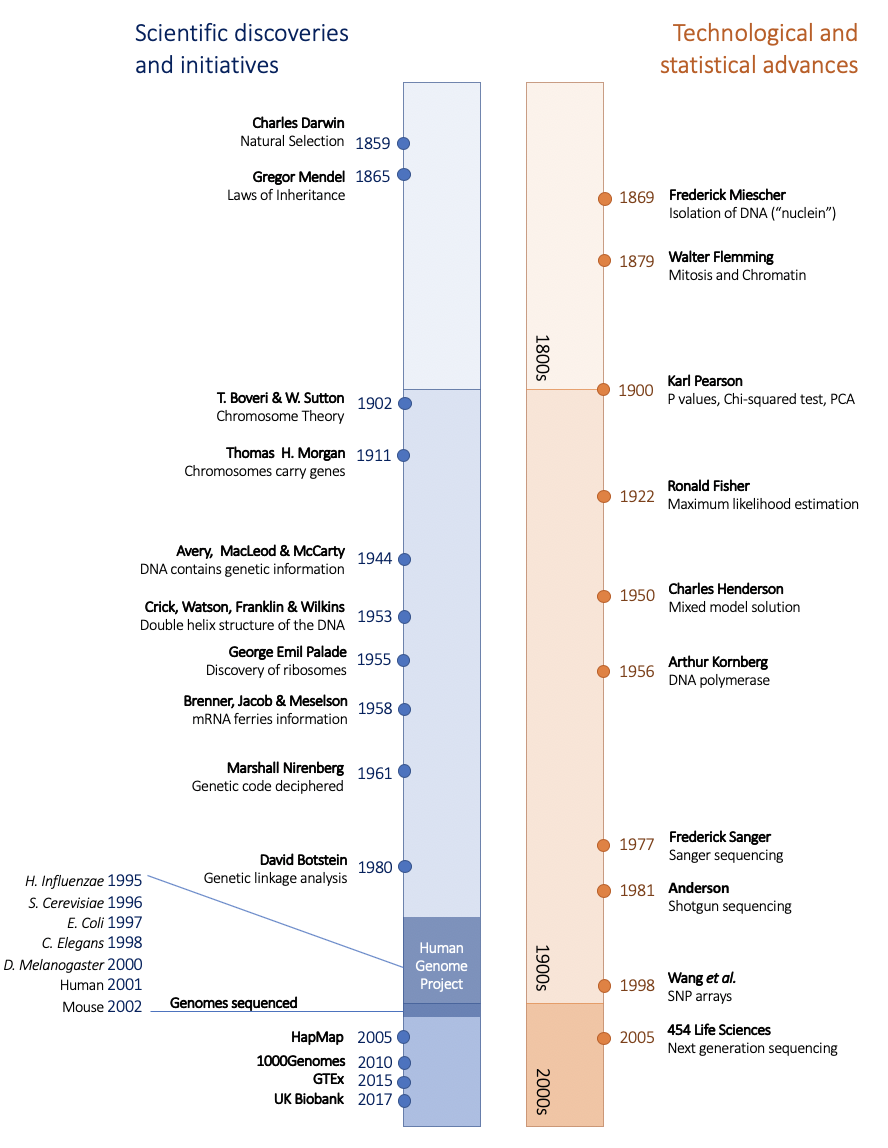
\includegraphics[width=15cm]{Chapter1/Fig/genetic_timeline_draft.png}
\caption[Genetic Timeline]{\textbf{150 years of genetics}.\\
% Key scientific discoveries in genetics and corresponding technological advancements.
A number of scientific discoveries, in combination with key advances in technology and statistical modelling, have led to the identification of thousands of genetic variants which are associated to complex and molecular traits \cite{nhgri2003genetic}.
Several fundamental contributions have been made, from Mendel's peas to the structure of DNA, to large databases cataloguing genetic variation of hundreds of thousands of individuals.
Here, I have attempted to highlight the key events that led to today's field of quantitative genetics in the GWAS and post-GWAS era.}
\label{fig:genetic_timeline}
\end{figure}

\subsubsection{Sequencing DNA}
\label{sec:dna_seq}

In terms of technology, one major leap in our understanding of the biological basis of genetic variation was the development of \gls{dna} sequencing, which allowed the nucleotide sequence of a DNA segment to be determined.
In the mid 1970s, two different \gls{dna} sequencing techniques were independently developed: the well known and still used Sanger chain-termination method \cite{sanger1975rapid, sanger1977dna} and a chemical sequencing method that has been almost forgotten, known as Maxam–Gilbert sequencing \cite{maxam1977new}.
The former, named after its developer Frederick Sanger, relies on \textit{in vitro} DNA replication by DNA polymerase, which had been isolated some twenty years prior by Arthur Kornberg and colleagues \cite{kornberg1956enzymic}.
The selective incorporation of `chain-terminating' dideoxynucleotides (ddNTPs)\footnote{either ddATP, ddCTP, ddGTP or ddTTP.
These nucleotides are missing a 3' -OH group, which is required for the formation of a bond between two nucleotides, causing DNA polymerase to stop the extension of DNA when a modified ddNTP is incorporated - thus the name chain-terminating sequencing.} alongside regular nucleotides during DNA synthesis, and the use of polyacrylamide gel electrophoresis to separate the resulting fragments, allows the sequence of an input DNA fragment to be determined. \\

Sanger sequencing eventually became the standard for \gls{dna} sequencing, and subsequent innovations led to the development of automatic sequencing machines able to sequence DNA fragments of about one kilobase (kb) in length. 
For sequencing longer stretches of \gls{dna}, a novel strategy named `shotgun sequencing' was developed \cite{staden1979strategy, anderson1981shotgun}. 
In shotgun sequencing, the long \gls{dna} of interest is randomly broken up into shorter \gls{dna} fragments which are cloned and sequenced separately. 
The occurrence of overlapping \gls{dna} fragments allows for the \textit{in silico} reconstruction of longer \gls{dna} fragments. \\

In 1995, the first genome of a living organism (the bacteria \textit{Haemophilus influenzae}) was sequenced and assembled by shotgun sequencing \cite{fleischmann1995whole}, shortly followed by that of another bacterium, \textit{Mycoplasma genitalium} \cite{fraser1995minimal}. 
The genomes of other model organisms were to follow in subsequent years - the budding yeast \textit{S. cerevisiae} \cite{goffeau1996life}, the bacterium \textit{E. coli} \cite{blattner1997complete}, the worm \textit{C. elegans} \cite{c1998genome}, the bacterium \textit{M. Tuberculosis} \cite{cole1998deciphering}, the fruit fly \textit{D. melanogaster} \cite{adams2000genome} and the flowering plant \textit{Arabidopsis taliana} \cite{kaul2000analysis}.
The first two human chromosomes (chromosome 22 and chromosome 21) were sequenced in 1999 and 2000, respectively \cite{dunham1999dna, hattori2000dna}, and the first draft of the entire human genome was published in 2001 \cite{lander2001initial, venter2001sequence} (see \textbf{page \pageref{sec:hgp}}).
The mouse genome was published in 2002 \cite{waterston2002initial}.

\subsubsection{Understanding the genetic basis of disease}
\label{sec:disease_genetic}

In parallel, along with the increasing understanding of the molecular structure of genes and the genome, scientists began to investigate the molecular basis of disease.
One of the first conditions to be linked to a genetic cause was alkaptonuria\footnote{a rare recessive condition that affects mainly the joints and causes unusual pigmentation.}, which in 1902 Garrod had identified  to follow the Mendelian rules of inheritance \cite{garrod1902incidence}.
In 1956, Vernon Ingram traced the cause of a disease to a genomic alteration for the first time: he discovered that sickle cell disease is caused by a chemical change in a hemoglobin protein \cite{ingram1963hemoglobins}. \\

Until the 21st century, success in identifying genetic factors responsible for human traits and diseases was predominantly through the use of genetic linkage studies, first proposed in 1980 by David Botstein \cite{botstein1980construction}.
These rely on the concept of linkage, first introduced by Morgan and his students: during meiosis, physically close genes remain `in linkage', whereas genes that are further apart are less likely to co-segregate due to recombination events.
When analysing a disease segregating\footnote{recurring within a family but without affecting all of its members.} in a family, linkage analysis involves i) identifying a genetic marker (with a known location) that is linked to the (unknown) disease gene and then ii) testing each of the nearby genes to determine the one that causes disease \cite{teare2005genetic}. 
Using this method, the first disease gene was mapped in 1983, when Gusella and colleagues linked a gene on chromosome 4 to Huntington's disease \cite{gusella1983polymorphic}.
Shortly after, in 1989, there followed a study from Francis Collins and others, identifying the genetic basis of cystic fibrosis as a single base deletion on chromosome 7 \cite{riordan1989identification}.
As of 2003, about 1,200 genes were linked to Mendelian traits \cite{botstein2003discovering}.\\

Mendelian disorders, as the name suggests, are those that follow the Mendelian laws of inheritance.
They are often called monogenic, as they are typically driven by mutations within a single gene with high penetrance (defined here as the probability of having a trait/disease given the predisposition score). 
Examples of such traits include X-linked muscular dystrophies, cystic fibrosis, Fanconi anaemia and phenylketonuria. 
Mendelian traits are typically rare in the general population but often cluster in families.
Genetic linkage analyses are best powered to discover these highly penetrant monogenic disease genes \cite{cardon2001association}.\\

In comparison, complex traits are typically common in the general population\footnote{The genetic architecture of human disease is captured on a spectrum \cite{manolio2009finding}, but can be broadly categorised as i) Mendelian (monogenic), ii) complex (polygenic) or iii) chromosomal (e.g. Down's syndrome).}.
They are driven by a combination of multiple genetic risk factors across the genome (hence the name polygenic), environmental risk factors, as well as interaction effects between genetic variants and environmental exposures (GxE).
These common, multifactorial diseases have a genetic architecture that is highly distinct from that of monogenic disease. 
They are known to be heritable (heritability estimates for most common diseases are estimated at 40-60\% \cite{manolio2009finding, prokopenko2009variants, kathiresan2008six, zeggini2008meta, harley2008genome}), but their full etiology contains both a genetic and an environmental component.
Consequently, it is the cumulative effect of many subtle genetic variants and environmental risk factors working in concert, that trigger disease onset.
Complex diseases include, for example, heart disease, type 2 diabetes, asthma, cancer, schizophrenia and Parkinson's disease.\\

Whilst there was some success in using linkage studies to identify genetic regions involved in common diseases\footnote{For example BRCA1 for breast and ovarian cancer  \cite{bailey2011linkage, miki1994strong}.}, genetic linkage studies in general proved underpowered to detect regions with significant linkage for complex traits and diseases \cite{bush2012genome, altmuller2001genomewide}. 
This was in line with the `common disease/common variant' (CD/CV) hypothesis \cite{bush2012genome, reich2001allelic}, which postulated that common traits are driven by genetic variation that is common in the population, i.e. multiple variants, each with low penetrance.
This hypothesis was described as early as 1996, and had already suggested that family-based linkage studies would be underpowered to detect variants with modest effects \cite{risch1996future}. \\

\phantomsection
\label{sec:ld}
Instead, it was proposed that the combined use of \gls{ld}\footnote{LD: the nonrandom allocation of alleles at nearby variants to individual chromosomes as a result of recent mutation, genetic drift or selection, manifest as correlations between genotypes at closely linked markers \cite{mccarthy2008genome}.} and population- (rather than family-) based studies would be more suitable \cite{risch1996future, jorde2000linkage} - thus practically proposing the design for \glspl{gwas} \cite{risch1996future}.
However, at the time, implementation of \glspl{gwas} was not possible, for two primary reasons.
First of all, the technology required to genotype thousands to millions of markers in a single experiment for the larger required sample sizes was not available \cite{risch1996future, visscher2012five}.
Secondly, the distribution and density of genetic polymorphisms across the genome, and the \gls{ld} between genetic variants across different populations, were unknown.\\

In some sense, population-based association studies can be viewed as an extension of family-based linkage studies, in which the population studied (derived from common ancestors) acts as an extended pedigree and a much greater number of meiotic recombinations will have occurred between the analysed samples.
As a consequence, \gls{ld} regions are much smaller than within pedigrees of close relatives, thus requiring a more dense panel of genetic markers to be examined \cite{cordell2005genetic}.

\subsubsection{The Human Genome Project}
\phantomsection
\label{sec:hgp}

In order to study genomic variation, and therefore its role in disease, it was necessary to generate a reference genome.
This was the goal of the \gls{hgp}, which aimed at sequencing the entire human genome.
The \gls{hgp} was 
% perhaps the first 
a 
major breakthrough that dramatically changed the landscape of genetics, and was described by United States President Clinton as “an epic-making triumph of science and reason” \cite{clinton2000remarks} at the announcement of its completion.
Driven by and a driver of technological breakthroughs in \gls{dna} sequencing and genotyping, the \gls{hgp} was a massive international undertaking and a truly collaborative effort; sequencing and analysis took place across twenty centers in six different countries (USA, UK, France, Germany, Japan, China) and took 13 years to complete, costing approximately \$2.7 billion \cite{lander2011initial}.
Led in the US by then NIH director Francis Collins and by founder of Celera Genomics\footnote{The company Celera Genomics was formed in May 1998, with the objective of sequencing much of the human genome in three years \cite{venter1998shotgun}.} 
Craig Venter, and with large contributions from the UK, in particular from the Sanger Institute directed by John Sulston (who had first sequenced the genome of \textit{C. Elegans}), the \gls{hgp} was announced as a joint US-UK statement on June 26th, 2000.
After a first publication in 2001, the project was truly completed on April 25th, 2003, on the 50$^{th}$ anniversary of the Watson and Crick paper describing the helical structure of \gls{dna}.\\

The \gls{hgp} provided the first map (obtained from the genomes of a small number of individuals) of the $\sim$3 billion bases in the human genome \cite{lander2001initial, schmutz2004quality, hattori2005finishing}, and revealed that human \gls{dna} consists of surprisingly few exons (1.1\% of the genome), whereas introns cover 24\% of the genome \cite{venter2001sequence, lander2001initial}. 
Additionally, the number of genes was found to be smaller than expected, with around 30,000 being identified in 2001, and circa 21,000 genes being the latest (still debated) estimate at the time that this thesis is written \cite{pertea2018thousands}. 
Additional breakthroughs in sequencing technologies have expanded and refined the reference genome, which now captures more than 92\% of the genome and provides a landscape of its genes \cite{lander2011initial}.\\

With a complete map of the human genome in place, genetic variants could now be identified as those bases discovered in an individual that did not match the (reference) base annotated in the human genome map. 
Common variants, i.e. variants with \gls{maf}\footnote{The frequency of an
allele at a genetic locus is the proportion of chromosomes in the study sample that carry that allele \cite{laird2010fundamentals}. 
For a biallelic variant (a variant for which only two possible alleles are observed in the population), the frequency of the less common (minor) allele is called the minor allele frequency (MAF).} larger than 5\%, were called \glspl{snp}. 
Previous studies had estimated that approximately 0.1\% (1 base per 1,000) of an individual's genome was a polymorphism \cite{wang1998large, li1991low, cargill1999characterization}. 

These SNPs were scattered across the genome and it was now time to describe what type of variants they were, where in the genome they were located, and what (if any) effect they had on global phenotypes.

\subsubsection{The International HapMap Project}

The International HapMap Project was the first effort of its kind to systematically catalogue genomic variation. 
Additionally, it aimed to characterise the LD structure of the human genome, which would make GWA studies feasible. 
The HapMap was officially started in October 2002 as a collaboration between research groups and private companies in Canada, China, Japan, Nigeria, the United Kingdom and the United States with the goal of developing a haplotype map (HapMap) of the human genome \cite{international2003international}.
By genotyping individuals of African (YRI), European (CEU) and East Asian (JPT, CHB) descent, in Phase I HapMap assembled a publicly available database of common variants (\gls{maf}>5\%) in global samples \cite{international2005haplotype}. 
The HapMap expanded rapidly. 
By Phase II (2007), the database contained 2.1 million SNPs from the four original populations \cite{international2007second}.
Phase III (2010) added genotyping from seven additional populations, for a total of over 3 million SNPs in 11 global ancestry groups\footnote{ASW (African ancestry in Southwest USA); CEU (Utah residents with Northern and Western European ancestry from the CEPH collection); CHB (Han Chinese in Beijing, China); CHD (Chinese in Metropolitan Denver, Colorado); GIH (Gujarati Indians in Houston, Texas); JPT (Japanese in Tokyo, Japan); LWK (Luhya in Webuye, Kenya); MEX (Mexican ancestry in Los Angeles, California); MKK (Maasai in Kinyawa, Kenya); TSI (Tuscans in Italy); YRI (Yoruba in Ibadan, Nigeria).} \cite{international2010integrating}.\\ 

The growing popularity of genetic association studies in parallel with the expansion of the HapMap effort paved the way for the last needed technological breakthrough: microarrays.
By knowing the genetic location of thousands of variants, commercial companies were able to develop so-called `SNP chips' \cite{meaburn2006genotyping, oliphant2002beadarray}, which allowed for genotyping at specific locations across the genome.
In parallel, the data generated by the HapMap project enabled calculation of the LD\footnote{Pearson's correlation coefficient squared, $r^2$, is commonly used} between SNPs within the genome, effectively describing the chance that two SNPs will be inherited together \cite{bush2012genome}.
This enabled the identification of haplotypes and thus a minimal set of SNPs that capture the majority of the haplotype diversity within a population, called `tag SNPs' \cite{international2003international}. 
The collective LD information gathered by academics in those years \cite{slatkin2008linkage, pe2006evaluating, otto2002resolving} allowed companies such as Affymetrix and Illumina to develop SNP arrays that contained 
these tag SNPs, effectively capturing information about common variation across a large percentage of the genome while only directly genotyping a few thousand SNPs.\\

\newpage

% % %********************************** % 1.1.7  **************************************
\subsection{Genome-wide association studies}
\label{sec:gwas}

The data generated by the International HapMap Project combined with development of appropriate chip-based microarray technology, which enabled simultaneous genotyping of more than one million SNPs, led to the first wave of \glspl{gwas} \cite{visscher2012five}.
\gls{gwas} are a hypothesis-free\footnote{bar the selection of SNPs on the chip. 
More recently, shallow DNA-seq has been increasingly used as an alternative, making the approach truly hypothesis-free.} approach to test for statistical association between the genotype frequency of common genetic variants (considered one by one across the genome) and a phenotype of interest \cite{mccarthy2008genome}. 
The development of GWAS was accompanied by great enthusiasm, and the hope that these studies could better our understanding of the genetic underpinning of human disease, leading to improvement of prognosis and acceleration of drug and diagnostics development. \\

Initially, \gls{gwas} focused on complex phenotypes with binary outcomes, using a case-control design (i.e. diseased vs healthy).
Then, for each SNP and binary trait, the association was evaluated using a Cochran–Armitage (trend) test, a $\chi^2$ test or a Fisher's exact test comparing the numbers of cases and controls when stratified by their alleles at the locus of interest. 
The first successful \gls{gwas} was published in 2002 on myocardial infarction \cite{ozaki2002functional}.
The same design was then applied in a landmark GWA study conducted in 2005 for age-related macular degeneration (AMD), using 96 cases and 50 healthy controls and testing for associations at $\sim$100,000 SNPs \cite{klein2005complement}. 
In 2007, the Wellcome Trust Case-Control Consortium (WTCCC) published a study where they performed \gls{gwas} on seven different common diseases, using 2,000 cases for each of bipolar disorder (BD), coronary artery disease (CAD), Crohn's disease (CD), hypertension (HT), rheumatoid arthritis (RA), type I and II diabetes (T1D, T2D) and a common set of 3,000 healthy controls, demonstrating the feasibility of the use of a shared set of controls across several traits \cite{wellcome2007genome}.\\

A year later, in 2008, the \gls{gwas} Catalog was founded to keep a record of all published \gls{gwas} and identified associations \cite{welter2014nhgri}.
As of September 2020, when I am writing this thesis, the \gls{gwas} Catalog includes 4,694 publications, describing 197,708 SNP-trait associations \cite{macarthur2017new}.\\

Over time, quantitative traits have become increasingly popular to use as phenotypes, in addition to binary traits.
These include continuous traits such as height, weight and blood pressure.
Furthermore, linear regressions and their derivations have become more popular methods to assess association, due to their flexibility to include covariates \cite{mccarthy2008genome}.
I describe these models in detail in the next chapter (\textbf{Chapter \ref{chapter2}}). 

\newpage

\gls{gwas} results are often visualised using a Manhattan plot \cite{mccarthy2008genome}, where the negative log p value (as a measure of significance) is plotted on the y axis, against the corresponding genomic position (ordered by chromosome and position) on the x axis (\textbf{Fig. \ref{fig:manhattan}}). 
Peaks on these plots represent loci (multiple variants in \gls{ld}) that display evidence of association with the analysed phenotype. 
Variants are deemed to be significantly associated with a trait if they exceed an appropriately chosen p value threshold. 

\begin{figure}[h]
\centering
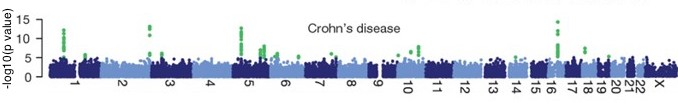
\includegraphics[width=15cm]{Chapter1/Fig/Manhattan_plots_CD_WTCCC_2007.jpg}
\caption[Manhattan plot]{\textbf{Manhattan plot}.\\
Manhattan plot for Crohn's disease (CD) from the WTCCC study \cite{wellcome2007genome}.
On the x axis are plotted the genomic positions of the SNPs tested, one chromosome after the next.
On the y axis are the association significance values.  
Alternating colours are used to distinguish chromosomes (odd numbered chromosomes -and chromosome X- are dark, even numbered chromosomes are light).
Highlighted in green are statistically significant SNPs (p value < $5 \times 10^{-8}$).}
\label{fig:manhattan}
\end{figure}

\subsubsection{From global traits to molecular traits}

Despite the success, the path from \gls{gwas} to biology is not straightforward, because an association between a genetic variant at a genomic locus and a trait is not directly informative of the causal mechanisms whereby the variant is associated with phenotypic differences \cite{visscher201710}. 
\gls{gwas} have robustly associated thousands of genomic loci with complex traits. 
However, the interpretation of the identified variants is often far from trivial: the true causal variants are often oscured by LD, and the genes mediating a variant's effect on the trait are rarely ascertainable from \gls{gwas} results alone, especially for non-coding variants, which account for the majority of \gls{gwas}-identified risk alleles \cite{manolio2009finding, gallagher2018post, wainberg2019opportunities}. 
Maps of regulatory annotations and connections in disease-relevant tissues, generated by projects such as ENCODE (ENCyclopdia Of DNA Elements, \cite{encode2004encode}) and Epigenome RoadMap \cite{kundaje2015integrative} can help the interpretation of these (putative) regulatory variants.
Additionally, molecular quantitative trait loci (QTL) mapping, where genomic variants are associated with changes in expression (eQTL \cite{schadt2003genetics}), chromatin accessibility (caQTL \cite{degner2012dnase}), DNA methylation (mQTL \cite{gaunt2016systematic}), histone modifications (hQTL \cite{grubert2015genetic}), or  protein level (pQTL \cite{melzer2008genome}), have added an interpretative layer to the molecular mechanisms associated with disease-associated variants. \\

In this thesis, I focus on gene expression, i.e., the transcriptome, as a molecular phenotype.
I use the next section (\textbf{section \ref{sec:eqtl}}) to describe key aspects of eQTL mapping.

% % %********************************** % 1.1.8  **************************************
\subsection{Expression quantitative trait loci}
\label{sec:eqtl}

\subsubsection{Mechanisms of the genetic regulation of gene expression}

During gene expression (or transcription), the genetic information stored in restricted portions of the \gls{dna} (genes) is used to produce RNA molecules. 
Next, during translation, the majority of RNA molecules are translated into  proteins. 
As we have seen, only approximately 1\% of the human genome is made up of protein-coding genes \cite{lander2001initial} whereas a large portion of the remaining sequence is thought to play a role in the regulation of gene expression \cite{encode2004encode}. \\

The impact of genetic variation on traits and disease is the consequence of perturbations to this complex molecular machinery.
An easily interpretable mechanism through which genetic variants may affect a phenotype is the direct alteration of the sequence and therefore functionality of the coded protein \cite{westra2014genome}. 
For example, sickle cell anaemia is caused by a \gls{snp} in the \textit{HBB} gene, which causes one amino acid substitution in the sequence of the corresponding protein \cite{laird2010fundamentals}. 
In alternative, genetic variation may affect the regulation of gene expression. 
One possible such mechanism would be the disruption of a specific sequence that affects the binding of proteins regulating the expression of a gene, for example a \gls{tf}. 
In this scenario, the regulatory variant is said to be acting in \textit{cis}.
An alternative mechanism is the alteration of the \gls{dna} structure, which in turn can affect the functionality of regulatory elements, and ultimately gene expression \cite{encode2004encode, kundaje2015integrative}. 
In this case the regulatory genetic variant is \textit{trans}-acting. 

\subsubsection{Mapping eQTL}
\label{sec:eqtl_map}

In the early 2000s, the new field of `genetic analysis of global gene expression' or `genetical genomics' \cite{jansen2001genetical} emerged, which applied traditional techniques of linkage and association analysis to thousands of transcript levels measured by microarrays \cite{rockman2006genetics}.
This was partly driven by the decrease in cost of high-throughput profiling of gene expression, which made it possible to measure gene expression levels in large numbers of individuals.
Genomic variants that were in this way associated with gene expression were termed \glspl{eqtl}. 
% \\
The first genome-wide maps of eQTL were performed in the early 2000s, using genetic linkage analysis, first in yeast \cite{brem2002genetic}, then in mammals, including humans \cite{schadt2003genetics}. 
A few years later, in 2007, the first modern eQTL studies using a GWAS-like approach were conducted in humans \cite{stranger2007population, dixon2007genome}. 
It soon became clear that gene expression levels are strongly heritable: for all human genes the average heritability (portion of phenotypic variation due to genetic variation) was estimated to be around 0.25 \cite{ricano2013mapping, dunham2012integrated, maurano2012systematic, westra2014genome}, making eQTL studies extremely popular.

RNA-sequencing\footnote{Today we would call this technique `bulk' RNA-sequencing as opposed to the more recent single cell RNA-sequencing; yet back then it was simply called RNA-sequencing, or `RNA-seq'.}, or RNA-seq, was a major breakthrough in the late 2000s and has been widely used since, substituting microarrays as the go-to technique to measure gene expression \cite{weber2015discovering}.
RNA-seq allows the measurement of the average expression abundance for each gene across a large population of input cells (\textbf{section 
\ref{sec:gene_expression}}).
The quantitative genetics field adapted quickly, and the first studies to perform \gls{eqtl} mapping using RNA-seq data to measure expression level were published back-to-back in 2010, by groups in Chicago and Geneva \cite{montgomery2010transcriptome, pickrell2010understanding}.
Today, (bulk) RNA-seq is the standard method to measure gene expression for eQTL mapping \cite{lappalainen2013transcriptome, gtex2015genotype, chen2016genetic}.
One of the advantages of RNA-seq compared to microarrays is that, in addition to the quantification of protein-coding genes, it also  gives insights about other RNA traits, including splicing, exon level and increasingly also transcript level (see also\textbf{ section 
\ref{sec:gene_expression}}).
As a consequence, splicing QTL (sQTL), can be mapped alongside standard (protein-coding) gene-level eQTL \cite{pickrell2010understanding, montgomery2010transcriptome}, as well as exon eQTL (eeQTL), transcript ratio QTL (trQTL) and miRNA eQTL, among others \cite{lappalainen2013transcriptome, bonder2019systematic}.
 
\subsubsection{\textit{Cis} and \textit{trans} eQTL}

An eQTL is a genomic locus that explains a fraction of the genetic variance of a gene expression phenotype (\textbf{Fig. \ref{fig:eqtl}}). 
As we have seen, regulatory effects on gene expression can usually be divided into those that act in \textit{cis} (on the same molecule of DNA) and those that act in \textit{trans} (on a different molecule of DNA, often through an intermediate).
To identify true \textit{cis} and \textit{trans} effects, differences in gene expression abundance between a pair of individuals can be compared to the level of \gls{ase} observed in their $F_1$ hybrid, similar to a classical \textit{cis-trans} complementation test \cite{mcmanus2010regulatory, goncalves2012extensive}. 
In this test, a real \textit{cis} effect would result in differential expression between the parents and corresponding \gls{ase} in the offspring. 
In contrast, a real \textit{trans} effect would result in no \gls{ase} in the offspring. \\

On the other hand, standard eQTL analysis involves a direct association test between markers of genetic variation with gene expression levels, without requiring any previous knowledge about specific \textit{cis} or \textit{trans} regulatory regions. 
This association analysis can be performed proximally or distally with respect to the gene. 
Conventionally, variants within 1 Mb (megabase) on either side of a gene's \gls{tss} are called \textit{cis} eQTL, while those at least 5 Mb downstream or upstream of the TSS or on a different chromosome were considered \textit{trans} acting \cite{nica2013expression, westra2014genome}.
Although this terminology is technically not accurate, it has been widely embraced by the eQTL mapping community, and I adopt this convention in this thesis. 


\begin{figure}[h]
\centering
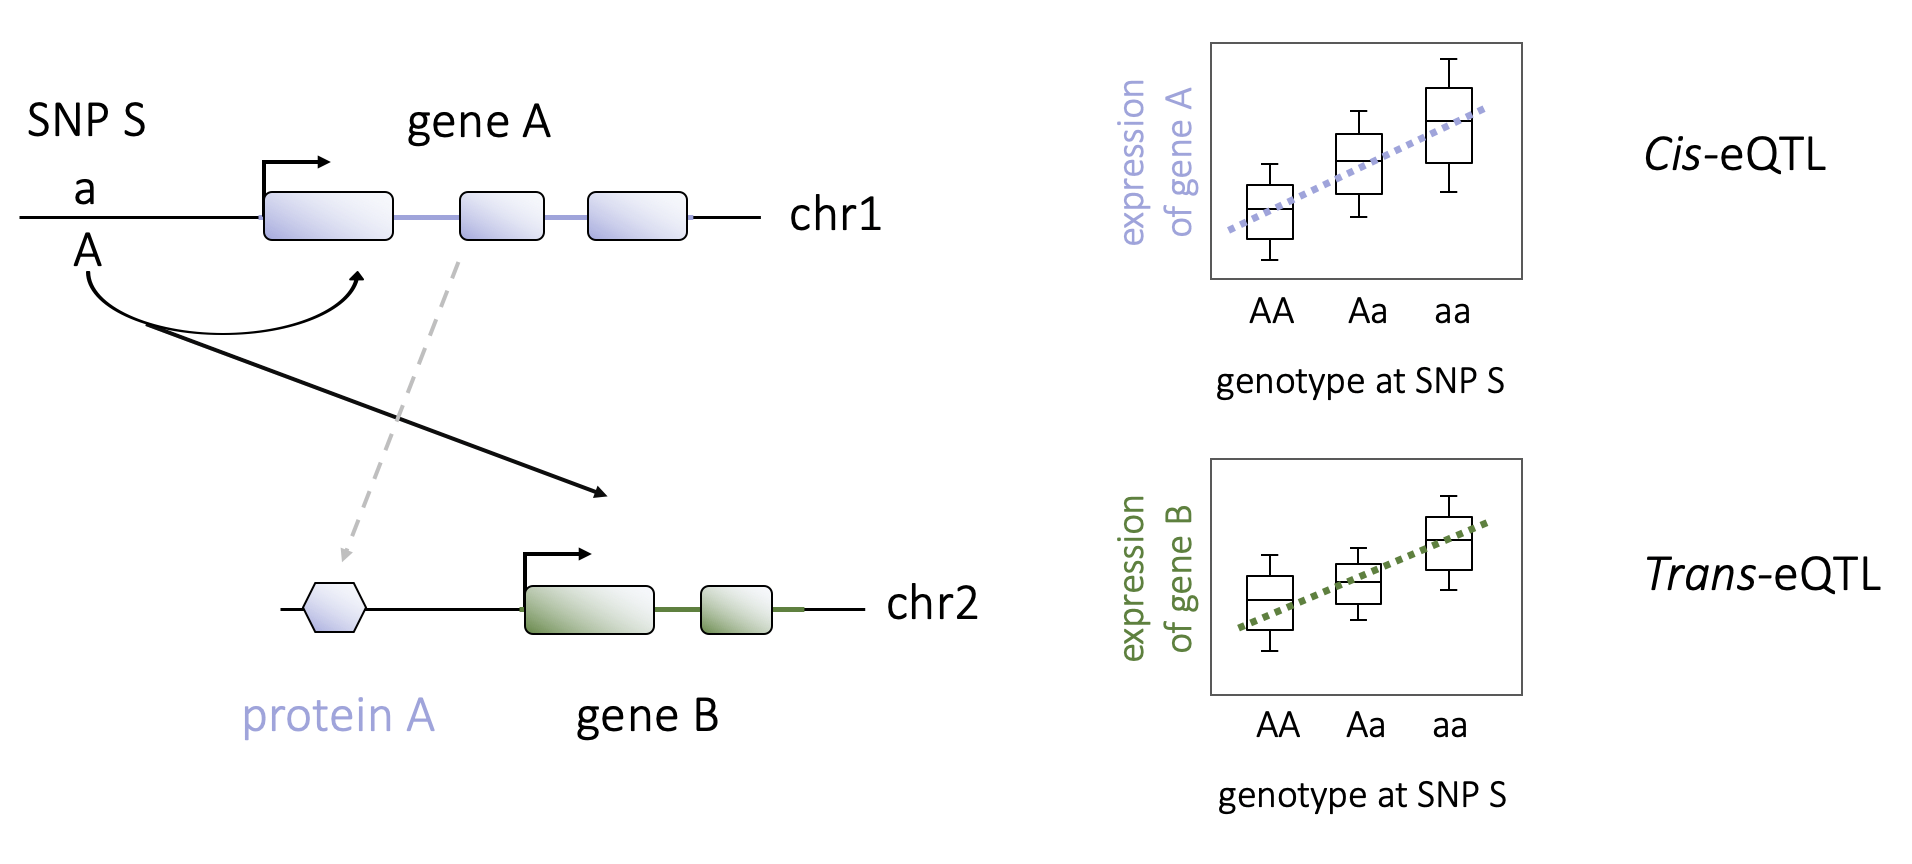
\includegraphics[width=15cm]{Chapter1/Fig/eqtl.png}
\caption[\textit{Cis} and \textit{trans} eQTL]{\textbf{\textit{Cis} and \textit{trans} eQTL}.\\
\textit{Cis} eQTL affect the expression of genes directly. 
\textit{Trans} eQTL, in contrast, affect the expression of typically more distant genes, often by first having a \textit{cis} effect on the expression of intermediate regulatory genes.
% On the right, the typical representation of eQTL using box plots.
Figure adapted from \cite{westra2014genome}.
}
\label{fig:eqtl}
\end{figure}


Typically, \textit{cis}-eQTL have a large effect size \cite{sherman2009systematic}, thus relatively modest sample sizes (from 80-100 samples) permit the detection of \textit{cis}-eQTL for thousands of genes \cite{stranger2007population, myers2007survey}.

\textit{cis}-eQTL effects appear to be mostly additive \cite{powell2013congruence}, and \textit{cis}-eQTL SNPs are often located close to the \gls{tss} of genes or within gene bodies \cite{vosa2018unraveling}. 
An eQTL effect sizes generally increases as the distance between the eQTL SNP and the gene's \gls{tss} decreases.
In contrast, the effect sizes of \textit{trans}-eQTL are generally small \cite{cookson2009mapping, grundberg2012mapping}. 
In addition, many more SNP variants need to be assessed, across all chromosomes, resulting in a much more severe multiple testing burden (see \textbf{section \ref{sec:multiple_testing}}).
Combined, these two aspects mean that much larger sample sizes are required to detect \textit{trans} eQTL.
As a result, the number of reported \textit{trans}-eQTL has remained small \cite{grundberg2012mapping} in comparison to the number of reported \textit{cis}-eQTL \cite{westra2014genome}.
In this thesis, I worked on datasets with relatively small sample sizes, and so only performed proximal (\textit{cis}) eQTL mapping.

\subsubsection{From tissue-specific to cell type-specific eQTL}
\label{sec:eqtl_celltype_specific}

Early studies mainly performed eQTL mapping in whole blood or blood-derived cells, due to sample accessibility \cite{stranger2007population, pickrell2010understanding}.
However, more recently, several studies have published eQTL derived from a number of normal human tissues \cite{myers2007survey, zhong2010liver,fu2012unraveling, nica2011architecture, dimas2009common, fairfax2012genetics, stranger2012patterns, schadt2008mapping, hao2012lung, innocenti2011identification}, motivated by the observation that gene expression levels vary considerably between different tissues and cell types \cite{su2002large}.
Perhaps most notable are those from the \gls{gtex} project, which set out to collect and analyse gene expression profiles across several primary tissues collected from post-mortem donors \cite{lonsdale2013genotype}.
Since the publication of their pilot study in 2015 \cite{gtex2015genotype}, several versions have been published \cite{gtex2017genetic, aguet2019gtex}.
The most recent version (v8) was released in 2019 and it includes data from 53 tissue types\footnote{Adipose - Subcutaneous, Adipose - Visceral (Omentum), Adrenal Gland, Artery - Aorta, Artery - Coronary, Artery - Tibial, 
Brain - Amygdala, Brain - Anterior cingulate cortex (BA24), Brain - Caudate (basal ganglia), Brain - Cerebellar Hemisphere, Brain - Cerebellum, Brain - Cortex, Brain - Frontal Cortex (BA9), Brain - Hippocampus, Brain - Hypothalamus, Brain - Nucleus accumbens (basal ganglia), Brain - Putamen (basal ganglia), Brain - Spinal cord (cervical c-1), Brain - Substantia Nigra, 
Breast - Mammary Tissue, Cells - Cultured fibroblasts, Cells - EBV-transfortmed lymphocytes,  Cervix - Ectocervix, Cervix - Endocervix, Colon - Sigmoid, Colon - Transverse, Esophagus - Gastroesophageal Junction, Esophagus - Mucosa, Esophagus - Muscularis, Fallopian Tube, Heart - Atrial Appendage, Heart - Left Ventricle, Kidney - Cortex, Kidney - Medulla, Liver, Lung,  Minor Salivary Gland, Muscle - Skeletal, Nerve - Tibial, Ovary, Pancreas, Pituitary, Prostate, Skin - Not Sun Exposed (Suprapubic), Skin - Sun Exposed (Lower leg), Small Intestine - Terminal Ileum, Spleen, Stomach, Testis, Thyroid, Uterus, Vagina and Whole Blood.} from 948 donors.
These studies have collectively identified \textit{cis} eQTL for the vast majority of human genes, emphasising their complex and cell type–specific nature, finding that 29\%–80\% of eQTL are cell type-specific \cite{gtex2015genotype, nica2011architecture, dimas2009common,  fairfax2012genetics}. \\

While eQTL from normal tissues provide valuable insights, tissues are constituted of multiple distinct cell types, each with specific gene regulatory profiles, as exemplified by the seminal work by Fairfax \textit{et al}., mapping eQTL in different blood-isolated cell types (monocytes and B cells \cite{fairfax2012genetics}).
Yet, apart from a few studies using purified cell types \cite{fairfax2012genetics, kasela2017pathogenic, naranbhai2015genomic} or deconvolution methods \cite{westra2015cell, venet2001separation}, eQTL datasets representing single primary cell types have been lacking \cite{zhang2018cell}.
Additionally, these methods are of limited use for less abundant cell types, and are dependent on accurately defined marker genes \cite{zhernakova2017identification}. \\
 
With the advent of single cell RNA-sequencing (scRNA-seq), eQTL mapping studies are now possible at the level of individual cells. 
scRNA-seq can be used to investigate rare cell types \cite{villani2017single}, and thus enables identification of cell type-specific eQTL in an unbiased manner. 
A first proof-of-concept study was published in 2013 on 15 individuals, where 92 genes were studied in 1,440 cells \cite{wills2013single}.
In 2018, the first genome-wide single cell eQTL mapping was performed in blood, on 45 individuals \cite{van2018single}.
For further discussion on performing eQTL mapping using single cell RNA-seq as opposed to bulk RNA-seq, see \textbf{Chapter \ref{chapter3}}.

\subsubsection{Context-specific eQTL}

In addition to cell type-specific eQTL, some effects of genetic variants on gene expression levels have been shown to manifest themselves only within cells that have been activated by a certain external stimulus (often called response eQTL \cite{fairfax2014innate, barreiro2012deciphering, kim2017genetic}) or only in cells under certain conditions \cite{yao2014sex} - both are sometimes referred to as `context-specific eQTL' \cite{westra2014genome}. 

\newpage

\subsubsection{Using eQTL to link genes to disease}
\phantomsection
\label{sec:eqtl_gwas}

Whilst useful in their own right to understand genetic regulation of gene expression across cell types and states, eQTL mapping can also be used for annotating variants associated with complex traits, as such variants are likely enriched for eQTL \cite{nicolae2010trait}. 
A recent study suggested that 2/3 of candidate complex trait mediating genes identified as eQTL are not the nearest genes to the GWAS lead variants, highlighting the utility of this approach in annotating GWAS loci \cite{zhu2016integration}. 
Importantly, GWAS variants are enriched in eQTL in a tissue-specific manner. 
For instance, whole blood eQTL are enriched with autoimmune disorder-associated SNPs but not with GWAS SNPs for bipolar disorder, or type 2 diabetes \cite{gtex2015genotype}. 
Thus, it is critical to use eQTL data from relevant tissues and cell types when following up GWAS loci for different diseases.\\

\textbf{GWAS-eQTL colocalisation}

Integrating eQTL maps with GWAS can identify potential molecular mechanisms underlying disease associations.
One such integration method consists in testing for `colocalisation' of a GWAS trait and a gene’s expression trait - i.e. test for whether the same variant is causal to both traits \cite{cannon2018deciphering}.
Intuitively, if it can be established that a causal variant for a GWAS trait and one for a gene’s expression are the same, this may suggest a regulatory role of the eQTL SNP in the pathway to the GWAS trait \cite{he2013sherlock, ongen2017estimating}. \\

However, simple overlap of GWAS and eQTL signals does not guarantee mechanism. 
First, the two variants may be two independent causal SNPs in LD with each other.
Second, eQTL are abundant \cite{lappalainen2013transcriptome}, with 48\% of common genetic variants estimated to act as eQTL for at least one gene \cite{liu2019abundant}, making the overlap between GWAS and eQTL signals possible by chance.
This motivated the development of formal statistical tests that estimate the probability of the overlaps between the two signals being due to chance - these are called colocalisation tests. \\

Early models \cite{plagnol2009statistical, wallace2012statistical, nica2010candidate} required full individual-level genotype data, which are seldom available \cite{cano2020gwas}.
More recently, Giambartolomei \textit{et al}. proposed a  colocalisation test (COLOC) which computes the odds of colocalisation compared to the null hypothesis using GWAS summary statistics \cite{giambartolomei2014bayesian}. 
Briefly, COLOC is a Bayesian statistical approach that tests for pairwise colocalisation of GWAS variants with eQTL, and generates posterior probabilities for each locus weighting the evidence for competing hypotheses of either no colocalisation or sharing of a distinct SNP at each locus \cite{guo2015integration}.
Since its release, COLOC has become a reference method for colocalisation testing. 
Alternative models for colocalisation include 
MOLOC (an expansion of COLOC to include multiple traits \cite{giambartolomei2018bayesian}).
JLIM \cite{chun2017limited}, 
HEIDI \cite{zhu2016integration}, 
Sherlock \cite{he2013sherlock},
eCAVIAR \cite{hormozdiari2016colocalization} 
and, most recently, `jointsum' \cite{deng2020powerful}.\\

\textbf{TWAS}

Colocalisation analyses effectively use genome-wide significant SNPs to nominate causal genes for complex traits. 
However, the majority of variants contributing to complex traits and diseases have not yet been identified, arguably because their effect sizes are too small to be detected at current GWAS sample sizes \cite{visscher201710}.
Theoretically, one may want to use tissue-specific gene expression, rather than genotypes, for association testing.
However, carrying out such studies is currently unfeasible, as it would require profiling gene expression across hundreds of thousands of individuals in both cases and controls, and across dozens of tissues \cite{cano2020gwas}.
Instead, transcriptome-wide association studies (TWAS) leverage eQTL information to predict (impute) the gene expression of the cases and controls from a GWAS, and then perform direct association of traits and genes - without directly profiling gene expression in every individual included in the GWAS \cite{wainberg2019opportunities}.
Several methods have been proposed, such as TWAS \cite{gusev2016integrative}, PrediXcan \cite{gamazon2015gene} and summary statistics-based Mendelian randomisation (SMR) \cite{zhu2016integration}. \\

In summary, both colocalisation and TWAS combine eQTL and GWAS catalogues with the aim to prioritise genes causally involved in complex diseases.
In particular, colocalisation analysis integrates association signals from GWAS and eQTL on a locus-by-locus basis to identify instances in which both traits share a causal variant. 
In contrast, TWAS leverages information from eQTL data to impute gene expression values for all individuals in a GWAS, and then associates genes directly to traits. 
The availability of eQTL catalogues from a wider variety of cell types, as well as of larger sample sizes, will improve gene prioritisation and translate GWAS results to refined sets of disease-causal genes \cite{cano2020gwas}.


\subsubsection{eQTL mapping in iPSC and iPSC-derived cells}

In addition to human primary tissues, \glspl{eqtl} have been described in human \glspl{ipsc} and \gls{ipsc}-derived cells (see \textbf{section \ref{sec:ips_genetics}}).
In the second part of this introduction (\textbf{section \ref{sec:human_ipscs}}), I describe the use of human \glspl{ipsc} as an \textit{in vitro} model for early human development and as a resource to generate donor-matched cell types and tissues that are impossible to access \textit{in vivo}.
Population-scale \gls{ipsc} derivation and differentiation provides an outstanding resource to investigate the role of genetic variants on expression in disease-relevant tissues and during development.


% ***********************************************************************************************************************************************************************************************************************************************************************************************************************************

\newpage

\vspace*{10px}

\textit{“It is not birth, marriage, or death, but gastrulation which is truly the most important time in your life.”}\\
\rightline{Lewis Wolpert, 1986}

\vspace*{5px}

% ***************************************************************
%************************ %Second Section %****************************************************************

\section{Human iPSCs to study cell differentiation}  %Section - 1.2
\label{sec:human_ipscs}  

Human \glspl{ipsc} and cells derived therefrom are the biological system I use throughout this thesis to study the effect of common genetic variants on expression during cell differentiation.
I use this section to provide some rudiments of human embryology and to describe the role of human stem cells in scientific research.
I focus especially on the \gls{ipsc} technology, which allows reprogramming of cells from easily accessible somatic tissues such as skin and blood to regain stem-cell like (pluripotent) properties and to be subsequently differentiated into virtually any desired cell type, when provided with the right stimuli.\\

In particular, in \textbf{section \ref{sec:history_developmental_biology}}, I provide a brief historical overview of the study of early development in humans and in \textbf{section \ref{sec:human_embryogenesis}} I describe the key stages of human embryology, which we attempt to mimic using \gls{ipsc}-derived differentiation protocols.
Then, in \textbf{sections \ref{sec:escs}} and \textbf{\ref{sec:cloning}}, I introduce the two key concepts of \glspl{esc} and \gls{scnt}, or somatic cloning.
\glspl{esc} are cells collected at a very early stage of the embryo's development that can be grown \textit{in vitro} to model development.
Somatic cloning, on the other hand, involves introducing the nucleus of a donor's somatic cell into an enucleated ovum which can either be implanted into a host and let develop, creating a `clone' for the donor; or, alternatively, grown \textit{in vitro} for research purposes.
Next, in \textbf{section \ref{sec:ipsc}}, I describe induced pluripotent stem cells (iPSCs), a technology that allows somatic cells to be reprogrammed to a pluripotent state, which can, in turn, be differentiated into virtually any differentiated cell types.
This allows the generation of \gls{esc}-like cells directly from a(ny) donor, bypassing the need for cloning. 
In this section, I will describe the technology and highlight advantages and challenges in the use of \glspl{ipsc} in biological research.
Finally, in the last section (\textbf{section \ref{sec:ips_genetics}}), I describe 
applications of human \glspl{ipsc} generated from many individuals to perform population-scale genetic analyses across a variety of \gls{ipsc}-derived cell types.

% %********************************** % 1.2.1  **************************************
\newpage

\subsection{From homunculi to developmental biology}
\label{sec:history_developmental_biology}

In the previous section, we learnt that DNA encodes all instructions of life, and that each one of us contains a mixture of genetic information from both parents, which is identically copied in every one of our cells.
But how do we go from one single cell containing our genetic fingerprint to a whole organism made of some 37 trillion highly specialised cells which differ in function and morphology and work together in harmony as a single organism?\\

Interest in the study of human development and the embryo has ancient origin.
We define an embryo as the first stages of development of a fertilised ovum in the uterus.
The word derives from the Greek \textepsilon\textmu\textbeta\textrho\textupsilon\textomikron\textnu \ (embryon, literally `young one').
Early embryology (from embryon and -\textlambda\textomikron\textgamma\textiota\textalpha, -logia, `study of') was first proposed by an Italian, Marcello Malpighi, who was a promoter of preformationism.
The theory of preformation believes that an embryo is contained in the semen (thus only derives from the father) and that it is essentially a preformed miniature infant (`homunculus') which just gets larger during development (\textbf{Fig. \ref{fig:early_embryology}}).\\

\begin{wrapfigure}{r}{0.6\textwidth}
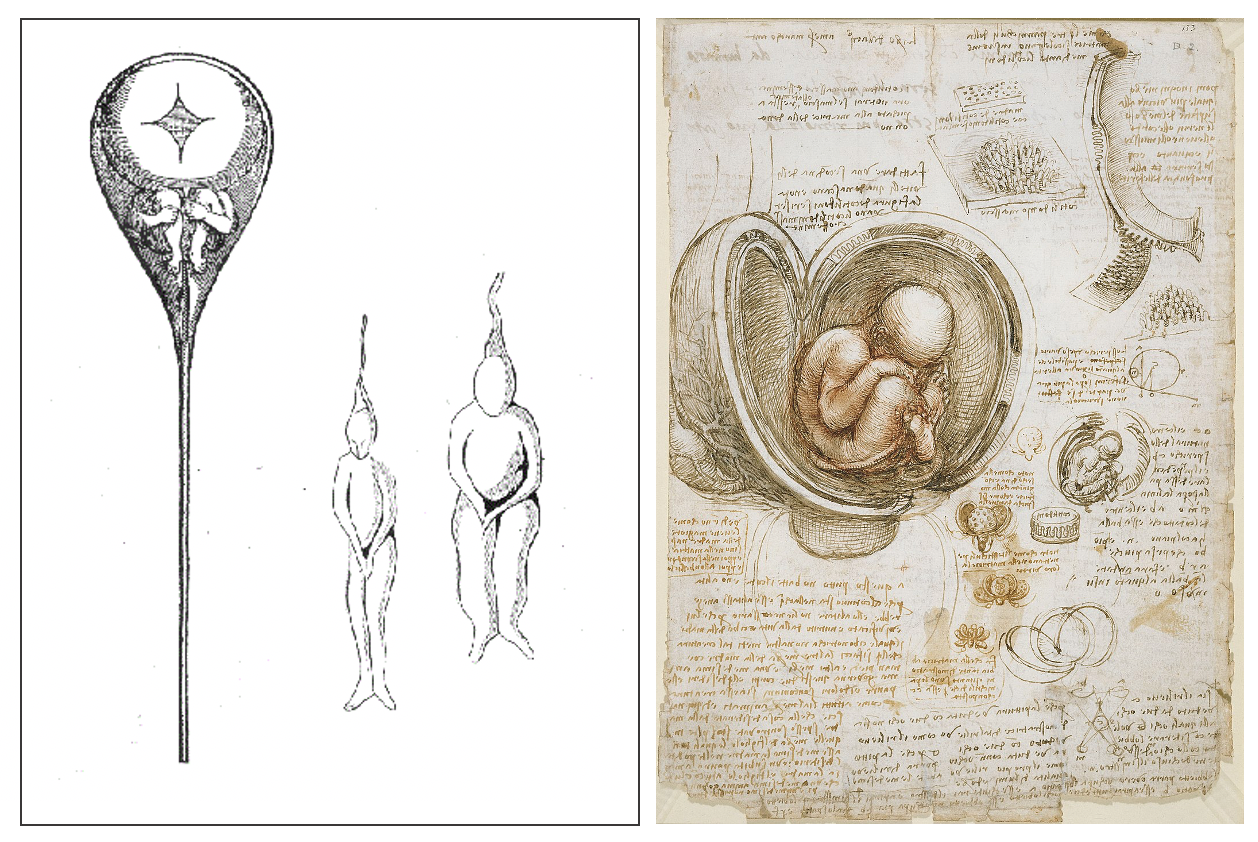
\includegraphics[width=9.5cm]{Chapter1/Fig/Early_theories_development.png}
\caption[Early theories of development]{\textbf{Early theories of development}.\\
Illustration of the two leading theories on human embryology before the 19$^{th}$ century.
Left, Illustration of Preformation: 
A tiny person (homunculus) growing inside a sperm, as drawn by Nicolaas Hartsoeker in 1695.
Right, Epigenesis: study of foetus deveopment by Leonardo Da Vinci, c. 1510.}
\label{fig:early_embryology}
\end{wrapfigure}

The alternative explanation for embryonic development was epigenesis, originally proposed by Aristotle approximately 2,000 years earlier. 
Much early embryology and support for epigenesis came from the work of Italian anatomists such as Aldrovandi and Leonardo da Vinci (\textbf{Fig. \ref{fig:early_embryology}}) in the Renaissance.
According to the theory of epigenesis, the shape of an animal emerges gradually from a relatively formless egg. 
Yet for centuries, most people believed in preformationism over epigenesis.
Only as imaging techniques improved during the 19th century, could biologists see that embryos take shape in a series of progressive steps, leading to epigenesis replacing preformation as the preferred explanation among embryologists.\\

Modern embryology developed from the work of Estonian-born Karl Ernst von Baer.
Von Baer is credited with discovering the mammalian ovum in 1827 and with becoming the first person to observe human ova.
Only in 1876 did Oscar Hertwig prove that fertilisation is due to the fusion of an egg and a sperm cell \cite{hertwig1875beitraege}.
Additionally, von Baer laid the foundation for the field of comparative embryogenesis in his `On the developmental history of animals', published in 1828 \cite{von1828entwickelungsgeschichte}.
In it, he formulated what became known as Baer's law of embryology.
In particular, he observed that large changes in embryo development precede more specific changes and that at a time in development embryos from different species look very similar, despite looking very different as adults.
Some of his ideas were later used by Darwin in his theory of evolution.
In his study of embryology, Von Baer discovered the blastula and formulated the germ layer theory (see next section, \textbf{section \ref{sec:human_embryogenesis}}).\\

\label{sec:carnegie_collection}
Human embryology as a scientific discipline is closely linked to the creation of human embryo collections \cite{yamada2015human, gasser2014rebirth, shahbazi2020mechanisms}. 
The seminal work of Franklin Mall led to the creation of the Carnegie collection in 1887, which includes more than 10,000 human embryo specimens, and established the basic staging criteria for the developmental classification of human embryos \cite{keibel1910manual}. 
Other collections were later created, such as the Kyoto collection, which today holds around 44,000 specimens \cite{nishimura1968normal}. 
Indeed, much of our current textbook knowledge of human development is derived from the early studies describing these samples.\\

The development of \gls{ivf} of human eggs \cite{edwards1969early, rock1944vitro, shettles1955morula}, followed by the development of conditions to culture these fertilised eggs for up to 5-6 days \cite{edwards1970fertilization, steptoe1971human}, allowed scientists to describe the dynamics of key morphological and genetic changes during early human development (see \textbf{section \ref{sec:human_embryogenesis}}).

In parallel, ever since the 1950s, with the helical structure of DNA being unraveled (see \textbf{section \ref{sec:double_helix}}), and with increasing knowledge in the field of molecular biology, developmental biology had emerged and was growing rapidly as a field of study that attempts to determine the interplay between morphological and gene expression changes during embryogenesis.
Indeed, development requires both mechanical changes in cell and tissue shape, which drive morphogenesis, as well as gene expression changes, which regulate cell fate decisions and tissue patterning \cite{niakan2013analysis, petropoulos2016single}. 
Mechano-chemical feedback at the molecular, cellular and tissue level coordinates this crosstalk and instructs tissue self-organisation \cite{hannezo2019mechanochemical}.

\newpage

\subsection{Human Embryogenesis}
\label{sec:human_embryogenesis}

I use this section to briefly outline the key steps of human embryogenesis as this is the system we aim to mimic \textit{in vitro} using differentiating human iPSCs.
Embryogenesis describes the first eight weeks of development\footnote{covering the 23 Carnegie stages.
The Carnegie system was based on work by Streeter \cite{streeter1942developmental} and O'Rahilly and Müller \cite{o1973developmental, o2010developmental} at the Carnegie Institution of Washington (based on the Carnegie collection, \textbf{page \pageref{sec:carnegie_collection}}).
The system is standardised and provides a unified developmental chronology of the vertebrate embryo.} after fertilisation, after which we generally refer to fetal development \cite{gilbert2008developmental}.\\

Thanks to technological advances in microscopy and \textit{in vivo} experiments in model organisms such as fruit flies and mice, we have learnt a lot about this process since the pioneering experiments of von Baer.
In particular, embryogenesis starts with a zygote, which is the single cell resulting from the fusion of gametes, an egg and a sperm cell; the fusion is known as fertilisation.
Then, the first 12-to-24 hours post-fertilisation are spent in cleavage, which consists of very rapid cell (mitotic) division and no growth \cite{khan2015human}.\\

At around day 3, cells start to get clumped together in a process called compaction \cite{iwata2014analysis}.
At this point (day 3/4), the 16-32 cell embryo is called the morula (which is the Greek word for mulberry), which will undergo blastulation \cite{wong2010non} (\textbf{Fig. \ref{fig:embryogenesis}}).
At around day 4, cells are still dividing, but they also begin to differentiate and develop specific forms and functions.
Two layers develop: the cells on the outer layer are called trophoblasts, and the cells inside are embryoblasts \cite{petropoulos2016single, niakan2013analysis}. 
Next, at around day 5, the embryoblasts clump even further into an inner collection of cells called the inner cell mass, which is pushed to a side of the sphere formed by the trophoblast.
The rest of the fluid-filled cavity is called the blastocoel and this conformation is called blastocyst.
This is also the time when the zona pellucida (a protective membrane that surrounded the egg cell and that was limiting the embryo's growth) begins to disappear, allowing the blastocyst to grow, change shape and start moving \cite{larsen2001human}.\\

The ability of the embryo to move allows the beginning of implantation: at around day 7, the embryo has now left the Fallopian tube and reached the uterus and attaches to its wall, the endometrium.
The trophoblasts divide and then fuse with the endometrium - initiating the process that will eventually build the placenta.\\

During the second week, these cells form another cavity called the amniotic cavity. 
At the same time, they start differentiating further into two layers: the epiblast (closer to the amnitioc cavity) and the hypoblast (closer to the blastocoel) \cite{khan2015human}. 

\begin{figure}[h]
\centering
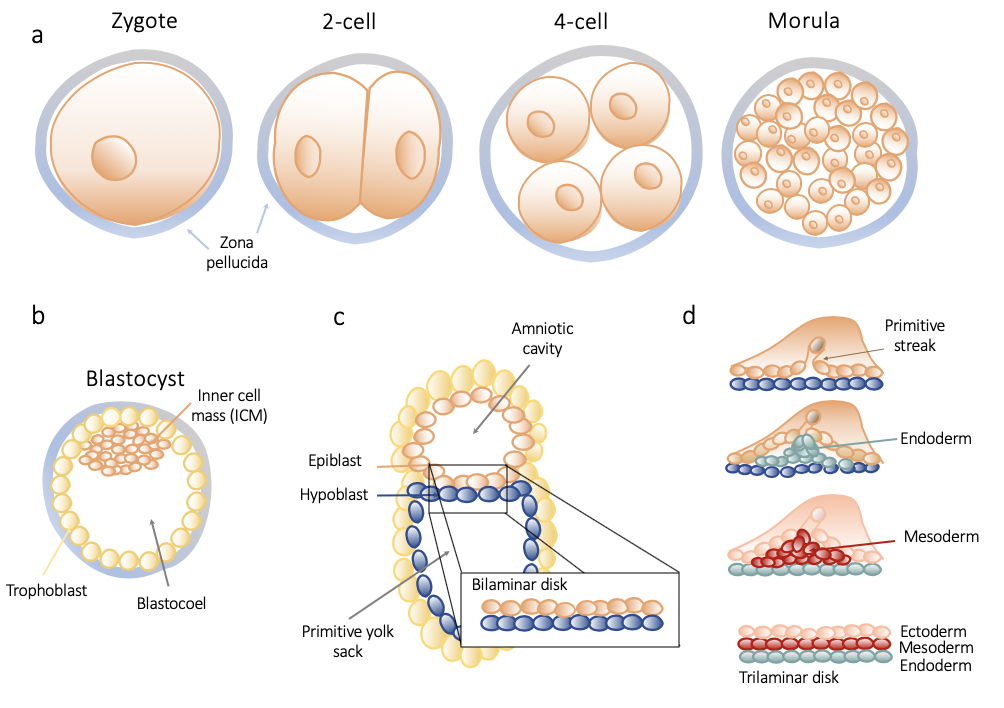
\includegraphics[width=14.5cm]{Chapter1/Fig/embryogenesis_til_gastrulation.png}
\caption[Human Embryogenesis]{\textbf{Human Embryogenesis}.\\
Early stages of human embryogenesis.
(a) From zygote to morula: stages of clevage.
(b) The blastocyst.
Cells divide and form an outer layer, the trophoblasts.
Inner cells also called embryoblasts get compacted and move to a side forming the inner cell mass (ICM), leaving a fluid filled cavity called the blastocoel.
(c) The formation of the bilaminar disk.
The ICM splits into the epiblast and hypoblast which distribute along the surface and result into two more cavities, the amniotic cavity and the primitive yolk sac, respectively.
(d) Gastrulation: from bilaminar to trilaminar disk.
The primitive streak forms and cells start to migrate moving down in between the epiblast and the hypoblast.
The endoderm, mesoderm and ectoderm form and are called the trilaminar disk.}
\label{fig:embryogenesis}
\end{figure}

Together, the epiblast and the hypoblast form the bilaminar disc \cite{hertig1956description}.
Only the epiblast contributes to the embryo, thus we do not discuss the hypoblast further (\textbf{Fig. \ref{fig:embryogenesis}}).\\

The next stage of early embryogenesis is gastrulation \cite{sheng2015epiblast}.
Famously called “the most important moment in your life” by Lewis Wolpert \cite{wolpert2015interview}, gastrulation is the process during which the three germ layers (endoderm, mesoderm and ectoderm) form.
At this stage, we call the cell mass a `gastrula'.
The first step of gastrulation is the formation of the primitive streak ($\sim$day 16).
The primitive streak determines the midline of the body, separating the embryo's left and right sides.
At this point, cells are moving down from the epiblast, ending up between the original epiblast layer and the hypoblast.
The first layer to invaginate descends the deepest and ends up closest to the hypoblast - this is the endoderm.
The next layer forms the mesoderm, and the remaining epiblast cells that continue to border the amniotic cavity are the ectoderm (\textbf{Fig. \ref{fig:embryogenesis}}).\\

The next stage is called neurulation (week 3-5).
Directly underneath the primitive streak, mesoderm cells form a thin rod, known as the notochord.
The notochord induces a change within the ectoderm above it, leading to the formation of the neural plate which then dives into the mesoderm to form the neural tube.
This is the end of what is called `early embryogenesis'.\\

Next, the germ layers start forming the various organs in a process called organogenesis.
Briefly, the endoderm forms the gastro-intestial tract, from which upper tract the lungs, the liver and the pancreas form. 
The tube itself forms the esophagus, the stomach, and the small and large intestines.
Second, the mesoderm forms some inner layers of the skin (endothelial cells), the muscles (including the heart), the bones, the kidneys, the bladder, ovaries and/or testis and blood cells.
Finally, the ectoderm forms the outer layer of the skin (epithelial cells), sweat glands and hair, and importantly our nervous system.
After eight weeks since fertilisation, we call the embryo a foetus, and fetal development begins.

\subsection{Human Stem Cells}
\label{sec:escs} 

% look up in humans
In mammals, roughly 50–150 cells make up the inner cell mass during the blastocyst stage of embryonic development, at around days 5–14 (\textbf{Fig. \ref{fig:embryogenesis}}). 
These have stem cell\footnote{stem cells are characterised by their self-renewing abilities and the `potency' to differentiate into more specialised cells.} capability, meaning that they can eventually differentiate into all of the body's cell types (making them `pluripotent').
Only the zygote is considered to be truly `totipotent' as it is able to form not only cells of the body (derived from the epiblast) but extra-embryonic tissues as well (from the hypoblast), which are necessary for the formation of a living organism.
Cells with stem-cell properties are still present in the adult body, and are called somatic or adult stem cells.
These are less potent than inner mass cells.
In particular, some adult stem cells have the ability to differentiate into a whole suite of cell types, and are called `multipotent'.
For example, this is the case for hematopoietic stem cells, which give rise to all the cell types of the blood and the immune system.
Other stem cells are more specialised, like epidermal stem cells, which are only able to differentiate into epidermal cells, or fibroblasts.
These are called `unipotent' (\textbf{Fig. \ref{fig:stem_cells}}).\\

\begin{figure}[htbp]
\centering
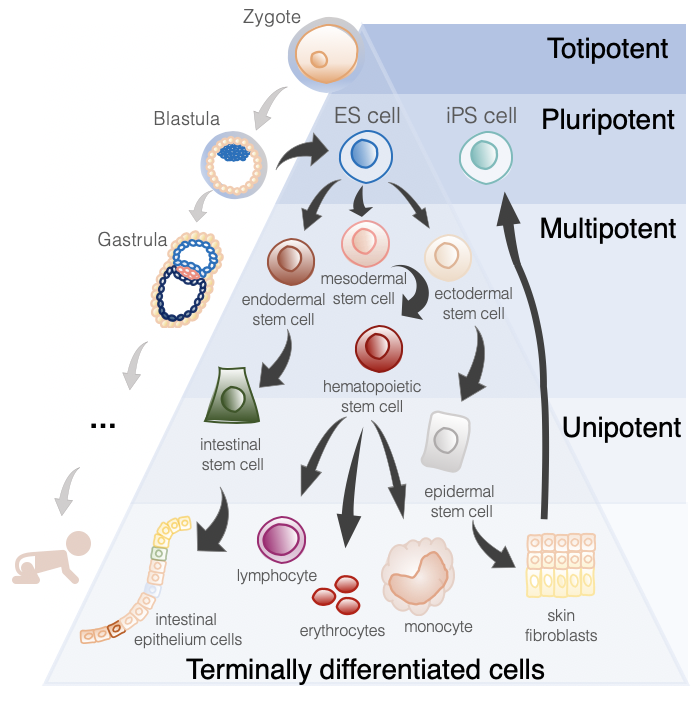
\includegraphics[width=16cm]{Chapter1/Fig/stem_cell_potency.png}
\caption[Stem Cells]{\textbf{The potency tree of stem cells}.\\
The spectrum of potency along human development: from the totipotent zygote to terminally differentiated cells.}
\label{fig:stem_cells}
\end{figure}

The existence of stem cells was first demonstrated by Canadian biologists Ernest McCulloch and James Till in the early 1960s.
Together with graduate student Andy Becker and senior scientist Lou Siminovitch their work was published in \textit{Nature} in 1963 \cite{becker1963cytological}.

\subsubsection{Embryonic stem cells}
\label{sec:esc_induction}

In 1981, \gls{es} cells were first isolated and successfully cultured using mouse blastocysts by British biologists Martin Evans and Matthew Kaufman \cite{evans1981establishment, martin1981isolation}.
In the 1990s, \gls{es} cell lines from two non-human primates, the rhesus monkey \cite{thomson1995isolation} and the common marmoset \cite{thomson1996pluripotent}, were derived, and these offered closer models for the derivation of human \gls{es} cells. 
The first \glspl{hesc} were finally isolated in 1998 by the American developmental biologist James Thomson \cite{thomson1998embryonic}.
Thomson and colleagues derived \gls{hesc} lines by culturing human blastocysts in a cocktail of growth factors and supporting mouse feeder cells.
Indeed as they first demonstrated, human inner mass cells, when isolated and cultured \textit{in vitro}, can be kept in the stem-cell stage and are known as  \glspl{hesc}. \\

Because they can proliferate without limit and can contribute to any cell type, human \gls{es} cells offer unprecedented access to tissues from the human body \cite{department2006regenerative}. 
As a consequence, \gls{hesc} lines held great promise for research purposes, as an \textit{in vitro} model for both human development and disease \cite{saha2009technical}.
First, embryonic stem cells have been used widely to improve our understanding of embryogenesis and development in general. 
Both in human and mouse, \glspl{esc} have been differentiated into a plethora of cell types.
Additionally, \glspl{esc} can be grown not only in a 2D culture but also in 3D structures, to better mimic the formation of organs (i.e. organoids \cite{clevers2016modeling, lancaster2013cerebral}) or even entire (early) embryos (the so called `gastruloids' \cite{van2020single2}). 
Additionally, they can be used as disease models and for \textit{in vivo} drug testing.\\

Second, \glspl{esc} could be used for cell replacement therapy, and, down the line, regenerative medicine \cite{kimbrel2015current}.
Indeed, not only do \glspl{esc} have the ability to self-renew indefinitely, but in theory they can also be differentiated into any cell type in the body, thus providing functional replacement or support to worn-out or dysfunctional cells and tissues and, in a future, replacing organ transplants entirely. \\

However, in order to isolate \glspl{esc} the embryo needs to be destroyed which, naturally, caused a big ethical debate.
Such ethical concerns caused the generation of \glspl{esc} to be reduced substantially or even made illegal in some countries.

Today, a number of lines have been isolated and frozen and are available for research.
Stem cell banks from a few countries provide (managed) access to several hundred \gls{hesc} lines including the UK Stem Cell Bank (139 lines) and the US NIH Human Stem Cell Registry (484 lines).
In total, it is estimated that there are between 800 and 1,000 \gls{hesc} lines available in the world which are, in the vast majority, derived from discarded IVF embryos \cite{isasi2009governing}. \\

In addition to the ethical controversies that the use of human embryos faces, which hinder the applications of human \gls{es} cells, it is difficult to generate patient- or disease-specific \gls{es} cells, which may be required for their effective clinical application \cite{yamanaka2007strategies}.


% %********************************** % 1.2.3  **************************************
\subsection{Nuclear cloning of somatic cells}
\label{sec:cloning} 
One early solution for the latter problem involved transplanting the nucleus of an adult donor cell in an enucleated oocyte in a process called nuclear cloning. \\

Nuclear cloning\footnote{The word `clone' comes from the Greek word for twig, as it was first applied in plants.}, also referred to as nuclear transfer or nuclear transplantation, denotes the introduction of a nucleus from an adult donor cell into an enucleated oocyte to generate a cloned embryo \cite{hochedlinger2003nuclear}.
This embryo has the potential, when implanted into the uterus of a female host, to grow into an infant that is a clone of the adult that provided the donor cell, in a process termed `reproductive cloning'. 
In alternative, the embryo can be explanted in culture, and give rise to embryonic stem cells that can differentiate into any adult cell type.\\

The first to perform nuclear cloning in animals was the British developmental biologist Sir John Gurdon. 
During his PhD in the Zoology department at Oxford, Gurdon worked on nuclear transplantation in a frog species of the genus \textit{Xenopus}.
In 1958, he successfully cloned a frog using intact nuclei from the somatic cells of a \textit{Xenopus} tadpole \cite{gurdon1962developmental}.
This critical study proved that eggs receiving transplanted nuclei from a more mature cell type could be differentiated, directly contradicting what was believed at the time \cite{king1955changes}. \\

The first cloned mammal was Dolly the sheep, born on July 5, 1996.
She was cloned by Keith Campbell, Ian Wilmut and colleagues at the Roslin Institute at the University of Edinburgh, using the process of somatic-cell nuclear transfer (SCNT) \cite{wilmut1997viable}.
Dolly had three mothers: one provided an unfertilised oocyte (cytoplasmic donor), another provided the nucleus (from a mammary gland cell\footnote{It is the use of a mammary gland as somatic cell source that motivated the name's choice: Dolly was named after country singer Dolly Parton, who is apparently famous for her breasts.}, nuclear donor) and finally a surrogate ewe hosted the embryo until its birth.\\

Following the successful cloning of Dolly the sheep and the pioneering work of Tada \textit{et al.}, who demonstrated somatic cloning by fusion of the somatic differentiated cells with \gls{es} cells \cite{tada2001nuclear}, many other species have been cloned, including pigs, cats, dogs, horses, camels and even macaques.
Combined, this work proved that somatic (differentiated) cells could be reprogrammed to a pluripotent state \cite{cowan2005nuclear}.\\

Until the early 2000s, the prospect of human cloned embryos explanted in culture was essentially the only envisoned way to generate patient- or disease-specific stem cells \cite{yamanaka2007strategies}.
However, application of \gls{scnt} in human cells proved extremely challenging \cite{fulka2013ups}\footnote{Only more recently has somatic cell nuclear transfer been successfully performed to generate human \glspl{esc} (NT-ESC), providing an alternative method to convert human somatic cells to a pluripotent state \cite{tachibana2013human}.}. 
In parallel, funding restrictions and ethical concerns around \glspl{hesc} provided the impetus to find alternative approaches for generating stem cells with the same degree of pluripotency.

% %********************************** % 1.2.1  **************************************
\subsection{Induced pluripotent stem cells}
\label{sec:ipsc}

The need to find both more ethical solutions and more effective ways of generating donor-specific stem cells  led to the generation of the first induced pluripotent stem cells (iPSCs).
Discovered in 2006 by Japanese stem cell researcher Shinya Yamanaka, iPSCs are somatic cells (originally mouse fibroblasts) which are reprogrammed into acquiring a stem-cell identity \cite{takahashi2006induction}.
Yamanaka has stated that it was the success of the cloning of Dolly the sheep that proved to him that reprogramming of somatic cells (in mammals) was possible.
The next year, the labs of Yamanaka and Thomson\footnote{The Thomson group had also isolated human ESCs for the first time in 1998, see \textbf{page \pageref{sec:esc_induction}}.} successfully generated \glspl{ipsc} from human somatic cells \cite{takahashi2006induction, takahashi2007induction, yu2007induced}, surpassing nuclear transplantation as the first step toward effective regenerative medicine and becoming the leading alternative to \glspl{hesc} for developmental research.\\

In 2012 Sir John Gurdon and Shinya Yamanaka were jointly awarded the Nobel Prize in Physiology or Medicine for their combined efforts in discovering that “mature cells can be reprogrammed to become pluripotent” \cite{nobel2012press} (\textbf{Fig. \ref{fig:ipsc_timeline}}).    

\begin{figure}[h]
\centering
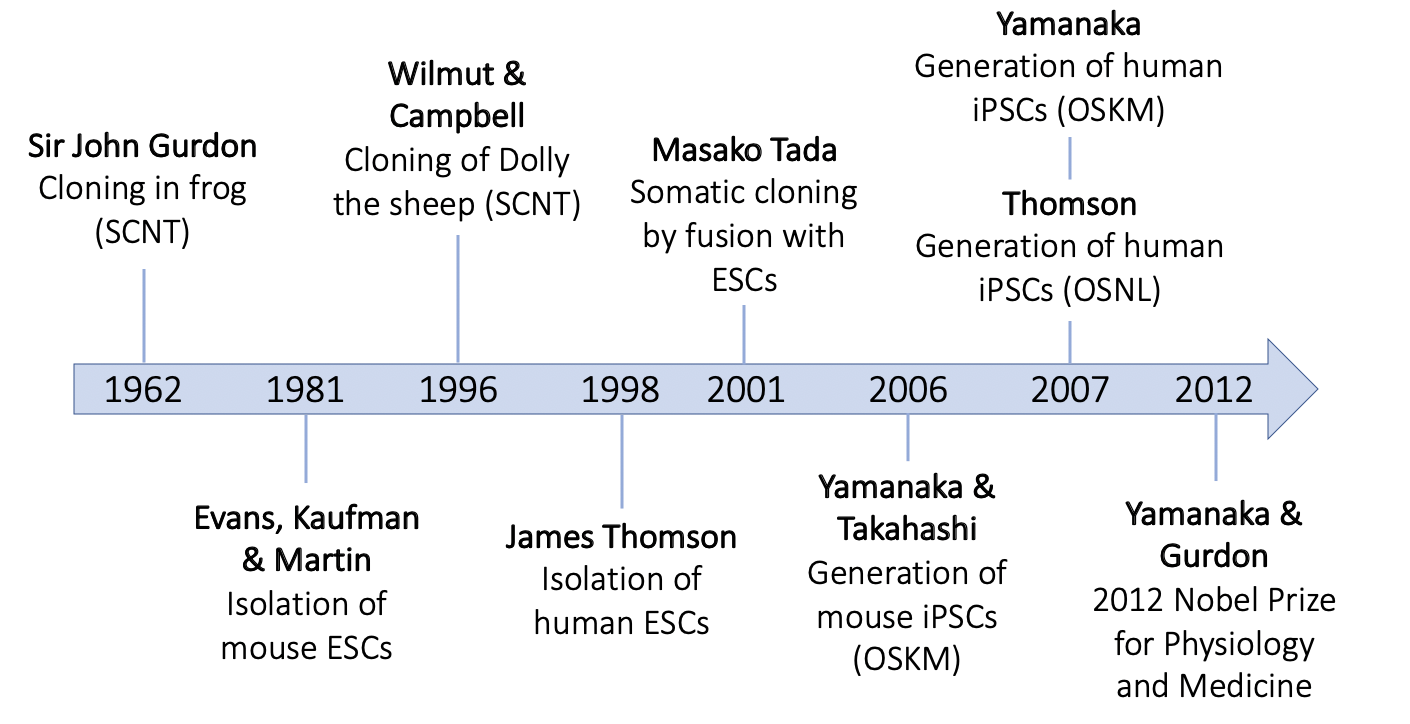
\includegraphics[width=15cm]{Chapter1/Fig/ipsc_timeline.png}
\caption[iPSCs timeline]{\textbf{Historical timeline of key events leading to the development of iPS cells}.\\
Key events including somatic cloning and isolation of ES cells that eventually led Shinya Yamanaka and colleagues to generate iPSCs in 2006 and Yamanaka to win the 2012 Nobel Prize for Physiology and Medicine alongside Sir John Gurdon.}
\label{fig:ipsc_timeline}
\end{figure}

\newpage

\subsubsection{Inducing pluripotency}

The generation of \glspl{ipsc} involves the reprogramming of differentiated somatic cells from readily accessible tissues (such as skin or blood) into a pluripotent state by the introduction of a cocktail of factors that are able to `reset' the transcriptional programme of the cells to an embryonic state \cite{saha2009technical}. \\

The induction of iPSCs (in mice) was first described in a seminal paper published in \textit{Cell}.
In it, Takahashi and Yamanaka first demonstrated induction of pluripotent stem cells from mouse fibroblasts (both embryonic and adult) by induction of four transcription factors, Oct3/4\footnote{also called Pou5f1.}, Sox2, c-Myc and Klf4, under ES cell culture conditions \cite{takahashi2006induction}.
In the paper, the authors demonstrate that \glspl{ipsc} exhibited similar morphology, proliferation properties and doubling times compared to \glspl{esc}.
Additionally, iPSCs expressed major ES cell marker genes like \textit{SSEA-1} and \textit{Nanog} and formed teratomas upon injection into immunocompromised mice\footnote{A teratoma is a non-malignant tumor comprised of a disorganised mixture of cells from all three germ layers. 
In a teratoma assay, putative pluripotent stem cells are implanted into an immune-compromised mouse where they may proliferate and differentiate to form a teratoma.}.\\ 

However, these `first generation' \glspl{ipsc} failed to generate adult chimerae\footnote{A chimera is a single organism composed of cells with more than one distinct genotype.
The name derives from Greek mythology, where a chimera was a fire-breathing monster that was part lion, part goat, and part dragon. 
To generate a chimera, \gls{ips} cells (e.g. with a gene-specific mutation) are injected into blastocysts, which are then transplanted into the uteri of pseudo-pregnant mice.
By breeding a chimeric mouse with a wildtype mouse and observing the corresponding phenotype, e.g. coat colour, one can assess the contributions of the \glspl{ipsc} to the germline \cite{okita2007generation}.} or contribute to the germline \cite{takahashi2006induction}, suggesting that the \glspl{ipsc} were only partially reprogrammed \cite{omole2018ten}. 
In 2007, Yamanaka and other laboratories modified the induction protocols to generate fully reprogrammed `second generation' \glspl{ipsc} that were competent for adult chimera and germline transmission \cite{maherali2007directly, wernig2007vitro, okita2007generation}.\\

A year later, the Yamanaka and the Thomson labs demonstrated, at around the same time, successful induction of pluripotent stem cells in human.
In the Yamanaka paper \cite{takahashi2007induction} human iPSCs were derived from adult human dermal fibroblasts using a retroviral system and using the same 4 factors used in mice, which later became known as the Yamanaka factors: Oct3/4, Sox2, Klf4 and c-Myc (or OSKM).
In their paper, published on the same day, the Thomson group also showed successful generation of human \glspl{ipsc}, using a slightly different technique: they used a lentiviral system to express the factors, and changed two of the inducing factors used: Oct4 and Sox2 remained, but the other two were replaced by Nanog and Lin28: this set of factors is sometimes called OSNL \cite{yu2007induced}.\\

In the next two years (2007-2009), the same technology was successfully applied by several groups and across a range of human cell types, including fibroblasts \cite{park2008reprogramming} and other somatic cell types, such as pancreatic $\beta$ cells \cite{stadtfeld2008reprogramming}, neural stem cells \cite{eminli2008reprogramming, kim2008pluripotent}, stomach and liver cells \cite{aoi2008generation}, mature B lymphocytes \cite{hanna2008direct}, melanocytes \cite{utikal2009sox2}, adipose stem cells \cite{sun2009feeder} and keratinocytes \cite{maherali2008high}, demonstrating the universality of cellular reprogramming \cite{omole2018ten}.

\subsubsection{Challenges in the use of iPSCs}
Yet for \glspl{ipsc} to fulfil their promise (that they are viable and possibly superior substitutes for ESCs in disease modeling, drug discovery, and regenerative medicine), several challenges on the road to their clinical application needed (and some still need) to be overcome.
First, very low efficiency was recorded: in the original Yamanaka paper, only 0.01–0.1\% \cite{takahashi2006induction} of the starting cells effectively exhibited pluripotency, and other initial reports did not exceed 1\% \cite{takahashi2007induction, okita2007generation, lowry2008generation}. \\

Second, the over-expression of oncogenes (genes that have the potential to cause cancer) such as \textit{c-Myc} and \textit{Klf4} during the generation of \glspl{ipsc} raised safety concerns.
Indeed, in the original report of germline-competent \glspl{ipsc}, $\sim$20\% of the offspring developed tumors that could be traced back to the reactivation of the \textit{c-Myc} transgene \cite{okita2007generation}. 
Furthermore, there is the risk of insertional mutagenesis due to virus-based delivery methods \cite{takahashi2006induction, takahashi2007induction, yu2007induced}. 
Finally, several studies have reported incomplete reprogramming, with cells maintaining some degree of `epigenetic\footnote{Epigenetics, from the Greek prefix epi- (meaning on top, around, in addition), refers to heritable changes of gene expression that do not involve variation in the genetic sequence of DNA.
For example, DNA methylation and histone modifications are common epigenetic changes.} memory' from their somatic cell of origin, which can lead to their biased differentiation potential into certain cell types depending on the donor cell source \cite{kim2010epigenetic, polo2010cell}.\\

Much progress has been made in the past decade to address these limitations and to improve the reprogramming technique, including the development of new methods to induce reprogramming. 
In the following sections I present an overview of the advances made to improve the reprogramming technique, and discuss methods for characterising \glspl{ipsc} in general. 

\subsubsection{Reprogramming factors}

Generating \glspl{ipsc} requires the introduction of pluripotency related factors into the somatic cell. 
The generation of \glspl{ipsc} by the Yamanaka and Thomson groups using different cocktails of transcription factors may suggest that different factors activate the same reprogramming pathway by reinforcing each other’s synthesis.
As a consequence, apart from the `fantastic four' OSKM transcription factors, Oct4, Sox2, Klf4, c-Myc and the alternative OSNL combination described by the Thomson group containing Oct4, Sox2, Nanog and Lin28 \cite{yu2007induced}, other factors, sometimes referred to as `reprogramming enhancers', have been found to increase reprogramming efficiency and iPSC quality \cite{takahashi2016decade}.
Those include other transcription factors, small molecules, microRNA’s (miR) and different culturing conditions. 


\subsubsection{Mechanisms of iPSC induction}

Several studies have described how the ectopic expression of OSKM in somatic cells induces the transition to a pluripotent state \cite{yamanaka2007strategies, brambrink2008sequential, stadtfeld2008induced, polo2012molecular, hansson2012highly, buganim2012single}. 
Based on these studies, we can now describe the order of events during the reprogramming process, which can be divided broadly into two waves or phases: an initial, stochastic early phase (phase 1) and a more deterministic and hierarchical late phase (phase 2) \cite{omole2018ten, takahashi2016decade, brouwer2016choices}.\\

During induction using the OSKM factors, the first transcriptional wave (phase 1) is mostly mediated by c-Myc and occurs in all cells, whereas the second wave (phase 2) is mostly targeted to `reprogrammable' cells, and involves a gradual increase in the expression of the Oct4 and Sox2 targets, leading to the activation of other pluripotency genes that aid in the activation of the pluripotency network. 
Klf4 seems to support both phases by repressing somatic genes during the first phase and facilitating the expression of pluripotency genes in the second phase \cite{buganim2013mechanisms}.\\

The two phases describe the mechanisms of reprogramming in the cells that successfully become pluripotent \glspl{ipsc}.
However, as we have seen, these are a rather small percentage of all transduced cells.
Three models, the elite, stochastic and deterministic models have been proposed to explain the reasons behind such low reprogramming efficiency \cite{omole2018ten}.
For more detail into these three models, I refer the reader to Takahashi \& Yamanaka \cite{takahashi2016decade}.

\begin{figure}[htbp]
\centering
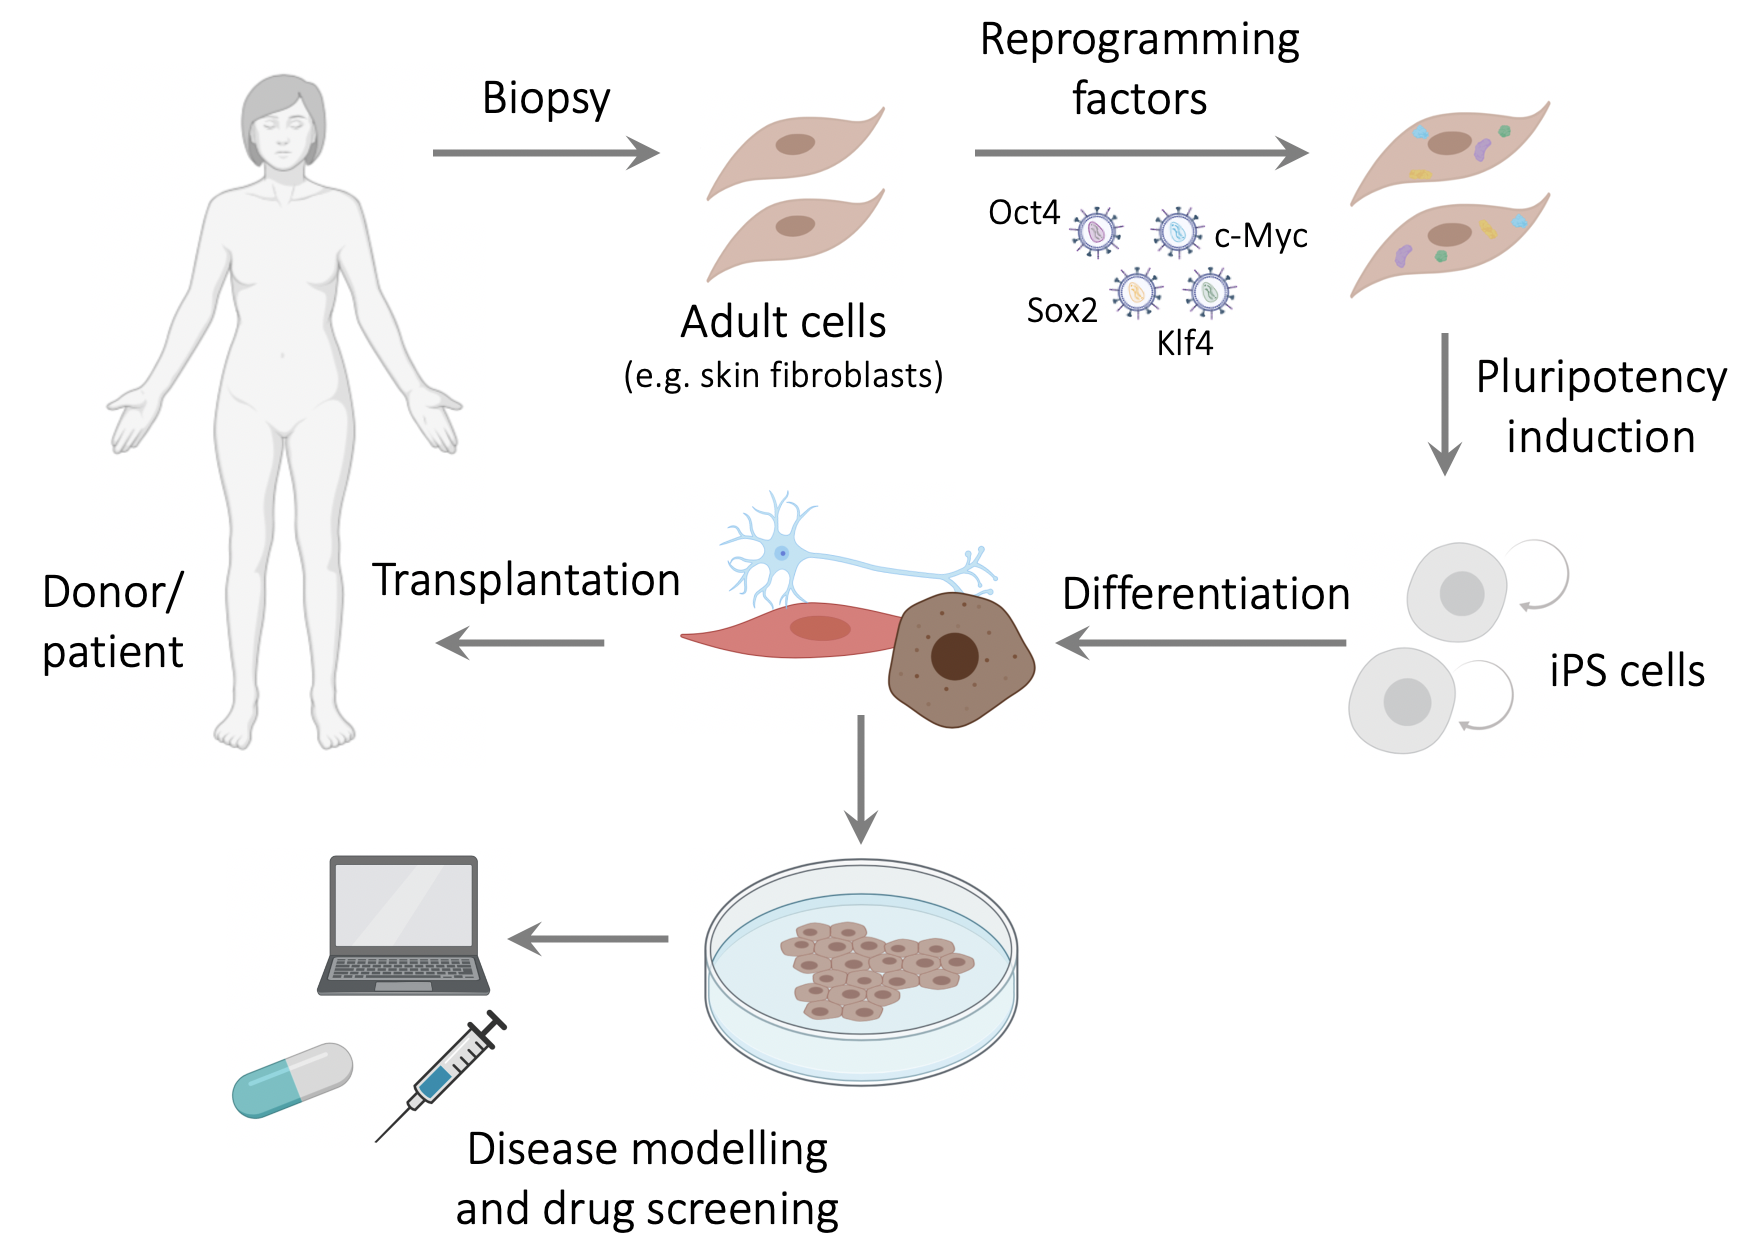
\includegraphics[width=14cm]{Chapter1/Fig/ipscs.png}
\caption[iPS cells]{\textbf{iPS cells - derivation and applications}.\\
The generation of iPSCs starts with a biopsy from, for example, the skin of an adult donor.
Adult cells, in the example fibroblasts, are then isolated and pluripotency is induced through four reprogramming factors, for example the Yamanaka factors: Oct4, Sox2, Klf4 and c-Myc (OSKM).
The factors can be delivered using a number of systems, see \textbf{page \pageref{sec:ipsc_delivery}}.
The resulting induced pluripotent stem cells (iPSCs) are self-renewing and are virtually indistinguishable from ESCs.
They can be subsequently differentiated towards other cell types, including disease relevant cell types, for example dopaminergic neurons for Parkinson's disease, or pancreatic beta cells for diabetes.
In the future, iPSC-derived cells might be used for cell therapy, i.e. they could be transplanted into the patient, with no risk of allogenic rejection.
In the meantime, iPSCs and iPSC-derived differentiations can be used to model development and disease, and to do compound screening and drug testing.}
\label{fig:ipsc}
\end{figure}


\subsubsection{Delivery methods}
\label{sec:ipsc_delivery}

A number of different methods have been used to deliver the reprogramming factors into somatic cells. 
These delivery methods can be categorised into two groups: integrative systems (involving the integration of exogenous genetic material into the host genome) and non-integrative systems (involving no integration of genetic material into the host genome). \\

Early methods to deliver the reprogramming factors were integrative.
These were mainly viral vectors, including retrovirus \cite{takahashi2006induction, takahashi2007induction, wernig2007vitro, okita2007generation, yamanaka2007strategies, maherali2007directly}, lentivirus \cite{yu2007induced, blelloch2007generation}, and 
inducible and 
excisable retrovirus \cite{soldner2009parkinson} or
lentivirus \cite{maherali2008high} systems. 
Overall, integrative delivery methods have higher reprogramming efficiency as compared to non-integrative methods, but they are less safe, due to the risk of insertional mutagenesis. \\

Indeed, the introduction of efficient, integration-free methods for cell reprogramming was crucial to reduce safety risks. 
These alternative non-integrative induction methods have been developed in recent years, and involve the transient expression of reprogramming factors, including the use of viral vectors (adenovirus \cite{stadtfeld2008reprogramming} and Sendai virus \cite{fusaki2009efficient, nishimura2011development}) and non-viral vectors, such as plasmids \cite{yu2009human, okita2008generation, okita2011more, jia2010nonviral}, transposons \cite{kaji2009virus, woltjen2009piggybac, yu2009human} synthetic mRNAs \cite{warren2010highly} and recombinant proteins \cite{kim2009generation}. \\

Because they are safer, the use of non-integrative methods is overall more appealing for iPSC generation and use in clinical settings.
Currently, episomal vectors, Sendai viruses and synthetic mRNAs are the most popular methods used for generating integration-free \glspl{ipsc}. 


\subsubsection{Somatic cell of origin}
\label{sec:ipsc_somatic_cell}

As for the cell source for reprogramming, somatic cells should preferentially be easily accessible, susceptible for reprogramming and the reprogramming process should ideally be highly efficient \cite{brouwer2016choices}. 
Several different human somatic cell types have been successfully reprogrammed; however, reprogramming efficiencies and kinetics vary between somatic cell types. 
Keratinocytes for example showed a 100 times higher reprogramming efficiency ($\sim$0.8\%) and were reprogrammed two times faster than skin fibroblasts under the same conditions \cite{aasen2008efficient}. \\

Today, human \glspl{ipsc} have been derived from a multitude of cell types \cite{doss2019current}, including dermal skin fibroblasts \cite{takahashi2007induction, yu2007induced}, adipocytes \cite{sugii2010human}, nucleated blood cells from peripheral blood \cite{loh2009generation, seki2010generation}, dental pulp \cite{yan2010ips},
keratinocytes from hair follicles \cite{aasen2008efficient} and
renal tubular cells from urine samples \cite{cao2018generation}.
However, approximately 80\% of human \glspl{ipsc} used in published studies are generated from fibroblasts \cite{takahashi2016decade}. \\

As mentioned above, the choice of cell source may also have consequences in terms of the epigenetic makeup of the \glspl{ipsc} generated.
Indeed, during the reprogramming process the somatic cells' epigenetic signature must be erased in order to adopt a stem cell-like epigenome.
These changes include chromatin reorganisation, DNA demethylation of promoter regions of pluripotency genes like \textit{NANOG}, \textit{SOX2} and \textit{OCT4}, reactivation of the somatically silenced X chromosome, and genome-wide resetting of histone post-translational modifications \cite{takahashi2007induction, maherali2007directly, wernig2007vitro, buganim2013mechanisms}.
If the reset is incomplete, cells may maintain some degree of `epigenetic memory' from their somatic cell of origin, which can lead to biased differential potential \cite{kim2010epigenetic, polo2010cell}.
However, it has been shown that their residual epigenetic memory diminishes as the cells are passaged in culture over a period of time \cite{ghosh2010persistent}.

\subsubsection{Characterising iPSCs}
\label{sec:ipsc_characterise}

As we have seen, reprogramming iPSC is a complex and not particularly efficient method.
As a consequence, it is important to carefully characterise the \glspl{ipsc} obtained after reprogramming \cite{brouwer2016choices} and establish criteria to evaluate the `quality' of iPSCs.
Different methods have been and should be used in combination to deeply characterise \glspl{ipsc}. 
First, the characteristic ESC-like morphology of \glspl{ipsc} is often used as an indication of their correct formation. 
\glspl{ipsc} can be observed as small cells with large nucleus/cytoplasm ratios that form tightly packed colonies with clear, sharp edges. \\

Second, \glspl{ipsc} are characterised by the expression of pluripotency markers including Oct4, Nanog, SSEA-3, SSEA-4, TRA-1-60 and TRA-1-81 \cite{boulting2011functionally}.
Additionally, bioinformatics tools, such as the PluriTest \cite{muller2011bioinformatic}, have been developed which use gene expression to assess the level of pluripotency. \\

In addition to morphological and gene expression considerations, \glspl{ipsc} can also be evaluated functionally by their differentiation potential.
Indeed, \glspl{ipsc} should be able to terminally differentiate into cells of all three germ layers (endoderm, mesoderm, ectoderm) - which can be evaluated through \textit{in vivo} teratoma formation assays or \textit{in vitro} differentiation through embryoid body (EB) formation.
Finally, since reprogramming influences the genetic and epigenetic make-up of the cells, \glspl{ipsc} should be carefully characterised for their genetic and epigenetic profiles.
Specifically, karyotyping is commonly used to evaluate genetic abnormalities in \glspl{ipsc}, i.e. to verify that cells are diploid. 
Additionally, if transgenes are used for reprogramming, it is important to verify that the expression levels of the transgenes are properly down regulated once the \glspl{ipsc} are formed. 
As for the evaluation of the epigenetic profile of the \glspl{ipsc}, DNA methylation patterns can be assessed. 
Since DNA methylation contributes to silencing of genes, it is important that the generated \glspl{ipsc} show DNA demethylation at key pluripotency genes (e.g., \textit{Oct4, Nanog, Sox2}), while genes specific to the donor somatic cell type become methylated and silenced \cite{brouwer2016choices, omole2018ten}. 

\subsubsection{Heterogeneity of iPSCs and between cell line variation}

An important aspect of iPSC biology is the  large variability observed between different iPSC lines and clones (even when derived from the same donor). 
This includes differences in terms of their differentiation capacity, epigenetic status, immunogenic and tumorigenic potential, maturation level, batch variability and co-occurrence of heterogenous populations of lineage subtypes and/or non-relevant cells as contaminating cell populations \cite{buganim2013mechanisms}.
This observed diversity, which is greater than what has been described in ESCs, can be explained by the residual epigenetic memory, genetic background and other characteristics acquired during reprogramming and differentiation \cite{kim2010epigenetic, polo2010cell, rouhani2014genetic}.
Naturally, understanding these sources of variable differentiation, particularly in terms of efficacy and safety, will be critical for the successful use of cell replacement therapies in the clinical setting \cite{buganim2013mechanisms}. \\

Thus, it is important to investigate sources of variable differentiation potential across lines, including lines derived from genetically distinct individuals.

\subsection{Applications of human iPSCs in genetics}
\label{sec:ips_genetics}

In contrast to ES cells, the use of which, as we have seen, raises important ethical concerns\footnote{as it involves the destruction of the embryo}, iPSCs can be derived from easily accessible tissues such as blood or skin, bypassing all such issues.
Because they are fairly easy to derive, they can be generated for individuals from all genetic backgrounds, including individuals carrying a genetic disorder of interest.
In the future, the iPSC technology opens the way to regenerative medicine where tissues can be re-generated with one's own cells thus avoiding the risk of immune rejection (when the body rejects a donor's allogenic organ as a foreign object).\\

In addition to the study of genetic disorders and the use for tissue regeneration, the iPSC technology can be applicable to basic biological research of human development and disease modeling.
Indeed, human \glspl{ipsc} have already been differentiated into a plethora of differentiated cell types, including neural stem cells \cite{d2014large}, 
cortical, dopaminergic and motor neurons \cite{shi2012human, kriks2011dopamine, karumbayaram2009directed}, astrocytes \cite{shaltouki2013efficient} and oligodendrocytes \cite{douvaras2014efficient} as well as  cardiomyocytes \cite{burridge2014chemically}, skeletal muscle cells \cite{maffioletti2015efficient},  vascular endothelial/smooth muscle cells \cite{patsch2015generation}, hepatocytes (liver cells) \cite{si2010highly}, pancreatic beta cells \cite{zhang2009highly} and  lung epithelial cells \cite{huang2014efficient}.\\

In recent years, as the iPSC technology became more established, iPSC lines have been derived from large cohorts, allowing deeper characterisation of these cells across multiple individuals.
This paved the way to the study of how common genetic variants affect gene expression in \glspl{ipsc}.
These large cohorts represent a resource which allows differentiation of a number of these lines and the interrogation of \glspl{eqtl} in derived differentiated cell types.

\subsubsection{HipSci and other human iPSC consortia}
\label{sec:HipSci}

The Human Induced Pluripotent Stem Cell Initiative (HipSci) \cite{kilpinen2017common} is the largest human iPSC cohort to date, and the results described in this thesis are all obtained using \gls{hipsci} lines.
The original goal of \gls{hipsci} was to generate a large, high quality reference panel of human iPSC lines for the research community to help deeply characterise these cells. 
All \gls{hipsci} donors are volunteers from the Cambridge area in the UK. 
Donors are for the vast majority of European descent, both male and female and across a range of ages (for healthy donors, [50-54]-[65-69]).
The majority of lines are derived from healthy donors, with small groups of diseased\footnote{Diseases included in \gls{hipsci} are monogenic diabetes, Bardet-Biedl syndrome, Usher syndrome, Hypertrophic cardiomyopathy and a few others, see \url{http://www.hipsci.org}.} samples.
For sample collection, primary fibroblasts from skin biopsies (from the inner upper arm to minimise somatic mutations due to sun exposure) were collected from consented research volunteers recruited from the NIHR Cambridge BioResource and iPS cell derivation was performed either using the Sendai reprogramming kit or episomal plasmids expressing the (human) Yamanaka factors: human (h)OCT3/4, hSOX2, hKLF4 and hMYC \cite{yu2009human}.
Following transfer to feeder free culture and expansion, each line was submitted to quality control and the criteria for line selection were: (i) level of pluripotency, as determined by the PluriTest assay \cite{muller2011bioinformatic}; (ii) number of copy number abnormalities; and (iii) ability to differentiate into each of the three germ layers \cite{kilpinen2017common}. \\


Additional iPSC consortia and large studies include
iPSCORE (a panel of fibroblast-derived iPSC lines from 222 ethnically diverse and sometimes related individuals \cite{panopoulos2017ipscore}), GENESiPS (a collection of 317 \gls{pbmc}-derived iPSC lines from 101 individuals \cite{carcamo2017analysis}), PHLiPS (containing PBMC-derived iPSC lines from 91 individuals of European and African-American ethnicity \cite{pashos2017large}), and Banovich \textit{et al} (a cohort of 58 lymphoblastoid cell line (LCL)-derived Yoruban lines, \cite{banovich2018impact}).

\subsubsection{eQTL mapping using iPSCs and iPSC-derived cells}

In 2017, the \gls{hipsci} consortium published a first paper, where they assessed iPSC lines through various assays, and mapped \glspl{eqtl} in 711 cell lines from 301 unique donors \cite{kilpinen2017common}.
At around the same time, another map of iPSC \glspl{eqtl} was published in \textit{Cell Stem Cell} \cite{deboever2017large}.
Most recently, a meta-study was published as the result of an effort to combine iPSC resources into the i2QTL consortium \cite{bonder2019systematic}.
Collectively, these studies have identified iPSC-specific eQTL, i.e. eQTL that function primarily in pluripotent cells.
A subset of these tagged disease-associated loci, suggesting that they are capturing molecular changes early in development which are not well captured by studies of differentiated primary tissues from adult individuals. 
Alternatively, iPSC eQTL may be capturing stem-cell like molecular mechanisms, which are similar to mechanisms active in cancer \cite{kilpinen2017common}. \\

In the last few years, \glspl{eqtl} have also been mapped in several iPSC-derived cell types.
These include iPSC derived- macrophages \cite{alasoo2018shared}, hepatocytes \cite{pashos2017large}, neurons \cite{schwartzentruber2018molecular} and cardiomyocytes \cite{strober2019dynamic, banovich2018impact}.
These \glspl{eqtl} promise to greatly improve our understanding of genetic regulation in cell types that we do not typically have access to, including cells at early developmental stages and cells that are difficult to isolate, such as neuronal cell types.
Combined with \gls{gwas} results (i.e. \textbf{page \pageref{sec:eqtl_gwas}}), they can contribute to our understanding of the genetic architecture of complex diseases by facilitating analysis in the relevant cell types, for example dopaminergic neurons for Parkinson's disease (\textbf{Chapter \ref{chapter5}}) or endoderm-derived (\textbf{Chapter 
\ref{chapter4}}) pancreatic beta cells for diabetes.

\newpage

\section{Thesis outline}

The overall aim of this thesis is to provide suitable computational methods for the identification of cell type and context-specific eQTL using single cell expression profiles, and explore their application across a range of human iPSC-derived cell types, using data from the \gls{hipsci} project.\\

Specifically, in \textbf{Chapter \ref{chapter2}}, I provide an overview of the use of linear and \glspl{lmm} for genetic association analyses, focusing on their application in \gls{eqtl} mapping.\\

In \textbf{Chapter \ref{chapter3}}, I describe best-practice approaches to perform \gls{eqtl} mapping using \gls{scrnaseq} profiles and demonstrate these methods on matched bulk and single cell expression of around 100 human \gls{ipsc} lines. \\

In \textbf{Chapter \ref{chapter4}}, I present a dataset of almost 40,000 cells from 125 human \gls{ipsc} lines differentiating to definitive endoderm, and demonstrate different approaches to \gls{eqtl} mapping using \gls{scrnaseq} data, identifying genetic variants that affect gene expression dynamically along differentiation and across other cellular states. \\

In \textbf{Chapter \ref{chapter5}}, I present a dataset of over one million cells from 215 human \gls{ipsc} lines differentiating to midbrain dopaminergic neurons.
We identify thousands of \glspl{eqtl} across a number of cell types and upon external stimulation.
In addition, we identify hundreds of colocalisation events with variants that are known to be associated with neurological traits and diseases.
Moreover, we investigate sources of variation in the capacity of individual cell lines to differentiate toward neurons.\\

Finally, in \textbf{Chapter \ref{chapter6}}, I conclude and discuss future directions.